\documentclass{memoir}
\usepackage{import}
\usepackage[utf8]{inputenc}
\usepackage[T1]{fontenc}
\usepackage{lmodern}
\usepackage{tabularx}
\usepackage{booktabs}
\usepackage{longtable}
\usepackage{titling}
\usepackage[svgnames]{xcolor}
\usepackage{enumitem}
\usepackage{tocloft}
\usepackage{subfiles}
\usepackage{graphicx}
\usepackage{float}
\usepackage{svg}
\usepackage{multicol}

\usepackage[centering, margin=1in]{geometry}
\usepackage{afterpage}

\usepackage[sorting=none,backend=biber,style=ieee]{biblatex}
\addbibresource{references.bib}

\usepackage{beuron}
\usepackage{libertine}
\usepackage{libertinust1math}
\usepackage{tcolorbox}

\usepackage{tipa}
\let\altdegree\degree
\let\degree\relax
\usepackage{siunitx}
\DeclareSIUnit\barn{b}

\usepackage[shortcuts]{extdash}

\usepackage{amsmath}
\usepackage{amsfonts}
\usepackage{amssymb}
\usepackage{mathrsfs}
\usepackage{cancel}
\usepackage{slashed}

\allowdisplaybreaks[1]

\usepackage[small, bf, hang]{caption}
\usepackage{subcaption}
\usepackage{url}

\usepackage[arrowdel]{physics}

\usepackage{tensor}
\usepackage[force]{feynmp-auto}
\usepackage{esint}

\usepackage{printlen}

\usepackage{hyperref}
\usepackage{tablefootnote}
\usepackage[noabbrev, nameinlink]{cleveref}
\definecolor{navyblue}{rgb}{0.0, 0.0, 0.5}
% this isn't working???
\hypersetup{
  colorlinks=true,
  linkcolor={red!50!black},
  citecolor={navyblue!50!black},
  urlcolor={navyblue!80!black},
}
\DoubleSpacing

\epigraphfontsize{\small\itshape}
\setlength\epigraphwidth{8cm}
\setlength\epigraphrule{0pt}


\begin{document}
\frontmatter
\thispagestyle{empty}
\pagecolor{navyblue}\afterpage{\nopagecolor}
\color{white}
\vspace*{10pt}
\begin{center}
\Huge\bfseries\scshape
\vspace*{10pt}
\rule{\textwidth}{1pt}
\vspace*{-9pt}
Introduction to $K_SK_S$ Physics at GlueX
\rule{\textwidth}{1pt}
\vfill
\begin{fmffile}{diagram}
\begin{fmfgraph*}(200,200)
    \fmfpen{thick}
    \fmfstraight
    \fmfleftn{i}{2}
    \fmfrightn{o}{3}
    \fmflabel{$p$}{i1}
    \fmflabel{$\gamma$}{i2}
    \fmflabel{$K_S$}{o2}
    \fmflabel{$K_S$}{o3}
    \fmflabel{$p$}{o1}
    \fmf{plain,foreground=white}{i1,t1}
    \fmf{photon,foreground=white}{i2,t2}
    \fmf{plain,foreground=white}{t1,t2}
    \fmf{plain,foreground=white}{t1,v1}
    \fmf{plain,foreground=white}{v1,o1}
    \fmf{phantom}{t2,v2}
    \fmf{phantom}{v2,o3}
    \fmffreeze
    \fmf{plain,label=$X$,foreground=white}{t2,v3}
    \fmf{plain,foreground=white}{v3,o3}
    \fmf{plain,foreground=white}{v3,o2}
    \fmflabel{$p$}{i1}
\end{fmfgraph*}
\end{fmffile}
\vfill
\Huge\bfseries\scshape
Nathaniel Dene Hoffman

Carnegie Mellon University
\end{center}
\color{black}
\clearpage
\begin{KeepFromToc}
    \setcounter{tocdepth}{2}
    \renewcommand{\contentsname}{Table of Contents}
    \tableofcontents
\end{KeepFromToc}
\thispagestyle{empty}
\mainmatter
\chapter{Introduction}
\section{A Brief History of Particle Physics}\label{sec:a_brief_history_of_particle_physics}

Since the days of the ancient Greeks, scientists and philosophers alike have been interested in the fundamental question concerning the composition of the universe. While some Greeks maintained that the world was composed of four indivisible elemental substances (fire, earth, air, and water)~\cite{Ross1925}, this was at best a guess by the early philosophers, who had no systematic mechanism with which to test their theory. Ironically, these philosophers struggled with a question to which modern physicists still have no answer: Are the building blocks of the natural world fundamental (indivisible)~\cite{Hardie1984}?

In 1808, John Dalton published a manuscript which described what is now called the "law of multiple proportions" after compiling several observations on chemical reactions which occur with specific proportions of their reactants. He anglicized the Greek \textit{atomos}, meaning ``not able to be cut'', into the word we are familiar with\textemdash ``atom''~\cite{Dalton1808}. Towards the end of the century, J. J. Thomson demonstrated that cathode rays could be deflected by an electromagnetic field, an observation which could not be explained by an alternative theory that the rays were some form of light~\cite{Thomson1897}. Instead, he proposed that these rays were made up of charged particles he called ``corpuscles'' (later renamed to the familiar ``electrons'')~\cite{Thomson1907}. Around the same time (between 1906 and 1913), Ernest Rutherford, Hans Geiger, and Ernest Marsden conducted experiments in which they scattered alpha particles through a thin metal foil, and, through an analysis of the scattering angles, concluded that a positively charged nucleus must exist at the center of atoms, surrounded by electrons~\cite{Rutherford1911}.

Over the next several decades, the nucleus was further divided into protons and neutrons\footnote{For the discovery of the electron and neutron, Thomson and James Chadwick won Nobel Prizes in Physics in 1906 and 1935, respectively. Rutherford won the 1908 Nobel Prize in Chemistry for his research in radiation. However, I want to emphasize that while I mention the ``big names'' here, there are many who contributed in relative obscurity.}~\cite{Masson1921,Chadwick1932}. In 1964, Murray Gell-Mann and George Zweig proposed a theory that protons and neutrons (and all other baryons and mesons) were in fact composed of smaller particles Gell-Mann called ``quarks''~\cite{Gell-Mann1964}. These particles, along with the electron-like family of leptons (including neutrinos), the gauge bosons, and the Higgs boson, first seen in 2012~\cite{Aad2012}, comprise elements of the Standard Model, a mathematical model which describes all the known forces and matter of the universe, with the notable exceptions (at time of writing) of gravity, dark matter, dark energy, and neutrino masses.

This thesis begins at a time when physicists are working hard to find gaps in this model, mostly by probing higher and higher ranges of energy. The experimental work being done at GlueX, however, resides in a lower energy regime, which we usually describe as ``medium energy physics''. As I will elucidate later in this manuscript, the strong force is non-perturbative in this regime, making direct calculations through the Standard Model all but impossible. However, since the advent of Lattice Quantum Chromodynamics (LQCD) in 1974~\cite{Wilson1974}, physicists have been able to make approximate predictions via computer simulations of the theory.

\section{Thesis Overview}\label{sec:thesis_overview}

Herein, I will focus on a particular portion of the Standard Model that dictates the strong interaction, viz. interactions between quarks and gluons, the mediating gauge boson of the strong force. Beginning with a discussion of the theory and history of $K_S^0$ (K-short) pair production in prior experiments, I will give a brief overview of the GlueX experiment. I will then outline some of the theoretical underpinnings and implications of glueballs to persuade the reader of the importance of this production channel in the larger scheme of GlueX.

Next, I will describe my own analysis, beginning with the layers of data selection which have been carried out to produce a clean sample of events. This will be followed by a discussion of the baryon contributions from excited $\Sigma^+$ hyperons, which were the original focus of my work when this project began. After removing these structures, we will use statistical weighting techniques to remove non-strange backgrounds from the dataset, focusing on the resonances which decay to $K_S^0K_S^0$.

I will then discuss the process of partial-wave analysis (PWA), modeling resonances, and selecting a waveset for my data. I will conclude with the results from fits of these models to the data, the implications of such fits, and the next steps which I or another particle physicist might take in order to illuminate another corner of the light mesonic spectrum.

\section{Motivation}\label{sec:motivation}

While this will be discussed in detail later, I believe it is important to emphasize the motivation for such a study of photoproduction of $K_SK_S$. While the majority of GlueX research concerns the search for hybrid mesons (mesons with valence gluons which contribute to their angular momentum, including ``exotic'' mesons with quantum numbers forbidden by $q\bar{q}$-only states), such mesons cannot be found in this channel, with the possible exception of glueballs, hypothetical bound states made entirely of gluons. Given a bound state of two spin-$\frac{1}{2}$ quarks with relative angular momentum $L$, total spin $S$ and total angular momentum $J$ (the eigenvalue of the operator $\hat{J}^2 = \hat{L}^2 \oplus \hat{S}^2$), we can define the parity operator $\hat{P}$ by its effect on the wave function of the system,
\begin{equation}
  \hat{P}\ket{\vec{r}} = \eta\ket{\vec{r}},
\end{equation}
where $\eta$ can be determined by noting that states of orbital angular momentum are generally proportional to a spherical harmonic in their angular distribution ($\ket{r,\theta,\varphi;LM} \sim Y_L^M(\theta,\varphi)$) and
\begin{equation}
  \hat{P}Y_L^M(\theta,\varphi) = Y_L^M(\pi-\theta,\pi+\varphi) = (-1)^LY_L^M(\theta,\varphi),
\end{equation}
so $\eta = (-1)^L$. The Dirac equation can be used to show that the intrinsic parity of quarks and antiquarks, when multiplied, yields a factor of $-1$, so
\begin{equation}
  \hat{P}\ket{q\bar{q};JLMS} = -(-1)^L.
\end{equation}

Similarly, the charge-conjugation operator $\hat{C}$ (also called C-parity) will introduce a factor of $(-1)^L$ because exchanging charges and other additive quantum numbers of a (neutral\footnote{For $\hat{C}$ to be Hermitian, and thus observable, acting it twice on a state should return the original state, so only eigenvalues of $\pm 1$ are allowed. Therefore, only states which are overall charge neutral are eigenstates of $\hat{C}$.}) quark-antiquark system is akin to reversing their positions under parity. If $\ket{S}$ is antisymmetric under C-parity, we should get an additional factor of $-1$, which is the case for the $S=0$ singlet. With the aformentioned $-1$ due to the intrinsic parity of the quarks and antiquarks, we find
\begin{equation}
  \hat{C}\ket{q\bar{q};JLMS} = (-1)^{L+S}
\end{equation}

Labeling states with the common $J^{PC}$ notation, it can then be shown that states like $0^{--}$, $0^{+-}$, $1^{-+}$, and $2^{+-}$ (among others) are not allowed states for $q\bar{q}$ mesons. As mentioned, the search for such states is a main focus of the GlueX experiment. However, since the particles we are concerned with decays to two identical mesons ($K_S$) which have a symmetric spatial wave function, and because these particles are mesons which follow Bose-Einstein statistics, the angular part of the total wave function must also be symmetric, i.e. $J = \text{even integers}$. Furthermore, because parity is conserved in strong decays, and the state of two identical particles is symmetric under parity, the decaying mesons must also have $P=+$. Finally, the strong interaction also conserves C-parity, and both kaons are neutral, so we can determine the $J^{PC}$ quantum numbers of the resonance to be $\text{even}^{++}$. There should be no overlap here with the aformentioned exotic mesons, but that does not mean the channel is not of interest to GlueX and the larger scientific community. Particularly, the lowest lying glueball states are predicted to not only share these quantum numbers, but exist in the middle of the mass range produced by GlueX energies~\cite{Morningstar1999}. To add to this, the spin-$0$ isospin-$0$ light flavorless mesons, denoted as $f_0$-mesons, may be supernumerary, either due to mixing with a supposed light scalar glueball or by the presence of a light tetraquark or hybrid states (or both)~\cite{Zyla2020}.

However, it would be an understatement to say that the $K_SK_S$ channel at GlueX is not the ideal place to be looking for hybrids, glueballs or tetraquarks. This is because, while we have excellent handles for reconstructing this channel, we have no ability to separate particles of different isospin with these data alone. This means that these $f$ states will be indistinguishable from their isospin-$1$ partners, the $a$-mesons. At first glance, it might seem like a model of the masses of these particles would make it easy to separate them, even if they remained indistinguishable between resonant peaks, but with broad states like the $f_0(1370)$ and states which sit right on top of each other (like the $f_0(980)$ and $a_0(980)$, which interfere with each other), there is likely no unique mass model which can distinguish all of the possible states without relying on data from other channels.

The silver lining is that, due to the GlueX detector's state-of-the-art angular acceptance~\cite{Adhikari2021}, we do stand a chance at separating spin-$0$ states from spin-$2$ states, and GlueX's polarized beam allows us to further understand the mechanisms at play by giving us some indication of the parity of the $t$-channel exchanged particle in the production interaction. We can also use this channel as a proving ground for more complex amplitude analysis involving a mass model, which could be extended to a coupled-channel analysis in the future.


\section{Past Analyses}\label{sec:past-analyses}
The present work is certainly not the first attempt to study $K_S^0$ pair production. The earliest published experiment with a similar final state dates back to 1961, where researchers at CERN measured 54 events which ended in a final state which included two neutral kaons\footnote{Since only $K_S^0$ eigenstates decayed inside the bubble chamber, while the longer lived $K_L^0$ would typically decay somewhere outside the chamber, these experiments infered a final state of $K_S^0K_S^0$. The same can be said for modern experiments, including GlueX.}. For the majority of the 1960s and 1970s, research into this final state was dominated by pion beam production off a proton target, aside from one kaon beam experiment in 1977 (see \Cref{tab:past-analyses}). In the 1980s, several collaborations at DESY began studying electron-positron collisions, which imply an internal virtual photon fusion as the production mechanism. These experiments are an important counterpoint to those involving hadrons, since the glueball does not couple to photons, so any intermediate glueball production in these reactions should be heavily suppressed~\cite{Acciarri2001}, although radial excitations of any glueballs should couple~\cite{Mathieu2009}. While the statistical power of these experiments was very small at first (relative to pion beam experiments), the L3 collaboration at LEP and Belle at KEKB provided larger data samples in the first two decades of the 2000s. Until this study, ITEP and BNL held the statistical lead in non-photon-fusion experiments, and we now present a dataset which is larger than both, even using the most restrictive selections of data.

There has only been one prior experiment, published by the CLAS collaboration in 2018~\cite{Chandavar2018}, which used photoproduction as a means of accessing this channel. While the ``golden channel'' for glueball production remains radiative $J/\psi$ decays to $K_S^0K_S^0\gamma$, since non-glueball intermediate processes converting charm quarks into strange quarks are suppressed, photoproduction could be effective at creating exotic hybrid states as well as glueballs via the photon's hadronic component or Pomeron exchange~\cite{Mathieu2009}. Additionally, the CLAS experiment did not utilize the polarized photon beam capability at JLab, but the current analysis at GlueX does, and this access to linear photon polarization can inform us of the parity exchanged in production of such exotic states. Our dataset is at least $5.7\times$ larger than what was achieved in the CLAS measurement.

\begin{table}
  \begin{center}
    \begin{tabular}{cccc}\toprule
      Channel & Collaboration & \# Events & Year\\\midrule
      $\pi^- p \to K_S^0 K_S^0 n$ & CERN/PS & 54 & 1961~\cite{DiCorato1961}\\
      $\pi^- p \to K_S^0 K_S^0 n$ & BNL & 19 & 1962~\cite{Erwin1962}\\
    $\pi^- p \to K_S^0 K_S^0 n$ & LRL & 66 & 1962~\cite{Alexander1962}\\
    $\pi^- p \to K_S^0 K_S^0 + \text{neutrals}$ & BNL & 374 & 1966~\cite{Crennell1966}\\
  $\pi^- p \to K_S^0 K_S^0 n$ & LRL & 426 & 1966~\cite{Hess1966}\\
  $\pi^- p \to K_S^0 K_S^0 n$ & LRL & 418 & 1967~\cite{Dahl1967}\\
  $\pi^- p \to K_S^0 K_S^0 n$ & CERN/PS & 2559 & 1967~\cite{Beusch1967}\\
  $\pi^- p \to K_S^0 K_S^0 n$ & ANL/ZGS & 1969 & 1968~\cite{Hoang1968} \& 1969~\cite{Hoang1969}\\
$\pi^- p \to K_S^0 K_S^0 n$ & CERN/PS & 4820 & 1975~\cite{Beusch1975}\\
$\pi^- p \to K_S^0 K_S^0 n$ & CERN/PS & 6380 & 1976~\cite{Wetzel1976}\\
$\pi^- p \to K_S^0 K_S^0 n$ & ANL/ZGS & 5096 & 1976~\cite{Cason1976} \& 1979~\cite{Polychronakos1979}\\
$K^- p \to K_S^0 K_S^0 + \text{neutrals}$ & CERN/PS & 410 & 1977~\cite{Barreiro1977}\\
$\pi^- p \to K_S^0 K_S^0 n$ & BNL/MPS & 1278 & 1980~\cite{Gottesman1980}\\
$\pi^- p \to K_S^0 K_S^0 n$ & BNL/MPS & 29381 & 1982~\cite{Etkin1982}\\
$e^+e^- \to e^+e^- K_S^0 K_S^0$ & DESY/TASSO & 100 & 1983~\cite{Althoff1983}\\
$K^-p \to K_S^0K_S^0 Y^*$ & ITEP & 283 & 1986~\cite{Bolonkin1986}\\
$\pi^-p \to K_S^0K_S^0 n$ & ITEP & 7156${}^{\dagger}$ & 1986~\cite{Baloshin1986}\\
    $\pi^- p \to K_S^0 K_S^0 n$ & BNL/MPSII & 40494 & 1986~\cite{Longacre1986}\\
  $e^+e^- \to e^+e^- K_S^0 K_S^0$ & DESY/PLUTO & 21 & 1987~\cite{Berger1988}\\
$K^- p \to K_S^0 K_S^0 \Lambda$ & SLAC/LASS & 441 & 1988~\cite{Aston1988}\\
$e^+e^- \to e^+e^- K_S^0 K_S^0$ & DESY/CELLO & 26 & 1988~\cite{Behrend1989}\\
$e^+e^- \to e^+e^- K_S^0 K_S^0$ & LEP/L3 & 62 & 1995~\cite{Acciarri1995}\\
$pp \to pp K_S^0 K_S^0$ & Fermilab/E690 & 11182 & 1998~\cite{Reyes1998}\\
$\pi^- p \to K_S^0 K_S^0 + \text{neutrals}$ & ITEP & 1000${}^\dagger$ & 1999~\cite{Barkov1999}\\
    $e^+e^- \to e^+e^- K_S^0 K_S^0$ & LEP/L3 & 802 & 2001~\cite{Acciarri2001}\\
  $\pi^- C \to K_S^0 K_S^0 + X$ & ITEP & 553 & 2003~\cite{Tikhomirov2003}\\
      $e^+e^- \to e^+e^- K_S^0 K_S^0$ & LEP/L3 & 870 & 2006~\cite{Schegelsky2006}\\
    $\pi^- p \to K_S^0 K_S^0 n$ & ITEP & 40553 & 2006~\cite{Vladimirsky2006}\\
    $e^+e^- \to e^+e^- K_S^0 K_S^0$ & KEKB/Belle & ???${}^\ddagger$ & 2013~\cite{Uehara2013}\\
    $\gamma p \to K_S^0 K_S^0 p$ & JLAB/CLAS & 13500${}^\dagger$ & 2018~\cite{Chandavar2018}\\
      $\gamma p \to K_S^0 K_S^0 p$ & JLAB/GlueX & 46928${}^\ast$ & 2025 (this analysis)\\\bottomrule
    \end{tabular}
    \caption{Summary of all (known) past analyses involving production of $K_S^0$ pairs. Note that this is possibly not exhaustive and does not include any studies which focus on decays of an intermediate state, i.e. $J/\psi \to \gamma K_S^0K_S^0$.\newline$\dagger$ - Estimated from plots.\newline$\ddagger$ - Reported as three orders of magnitude larger than LEP's result from 2006, but an exact count was difficult to estimate.\newline$\ast$ - Weighted number of events with KinFit $\chi^2_\nu < 3.0$, the standard selection used in this analysis (see \Cref{subsub:kinematic-fit,sec:data-selection}).}\label{tab:past-analyses}
  \end{center}
\end{table}

\chapter{Experimental Design and Data Selection}
\section{The GlueX Experiment}
\subsection{The GlueX Kinematic Fit}
\section{Data Selection for the $K_SK_S$ Channel}
\subsection{Fiducial Cuts}
\section{sPlot Weighting}
At this stage in the analysis, we have no more simple cuts which can improve the signal-to-background ratio in the dataset, but we know there must still be background remaining, as is indicated by the excess events with small kaon rest-frame lifetimes seen in \Cref{fig:rfl-pre-splot}. In this figure, we see that one of the intrinsic properties of a $K_S^0$, its well-known lifetime around $\SI{89.54}{\pico\second}$, is not present in the data. Rather, we seem to have at least two exponential slopes in the rest-frame lifetime distribution of each kaon, one which is close to what we see in signal Monte Carlo, and another which is similar to the $4\pi$ background Monte Carlo. The $K_S^0$ lifetime comes from the fact that it contains a strange quark but decays to two non-strange mesons, and a weak interaction is required for this to occur. While we might not know the exact process which creates the $4\pi$ background, we can assume a strong interaction produces the pions, which should happen several orders of magnitude faster than the $K_S^0$ decay. Due to the resolution of the detector, we still expect these events to appear to have some non-zero distribution in rest-frame lifetime when we mistakenly interpret pairs of pions as kaons, but it will be vastly different from that of the signal. Rather than cut out the low-lifetime events (greatly reducing the $K_S^0$ signal which also peaks at zero), we now turn to a more elaborate method of separating the signal from this potential background influence called sPlot~\cite{Pivk2005}\footnote{This is stylized as ${}_s\mathcal{P}lot$ in the original paper, but I find this tedious to type and to read.}, a weighting scheme which roughly weights each event by the probability of it coming from the signal or background distribution. However, na\"ively weighting by probability (a method dubbed ``inPlot'') can cause issues which can fortunately be easily corrected. We begin by giving a basic explanation of inPlot before describing the sPlot correction.

\begin{figure}
  \begin{center}
      \includesvg[width=0.8\linewidth]{ext/analysis/plots/rfl_combined_pz_masscut_chisqdof_3.0_mesons_None_None.svg}
  \end{center}
  \caption{The rest-frame lifetime of kaons in data, signal Monte Carlo, and background Monte Carlo. The data distribution clearly contains two exponential slopes: a peak which resembles the $4\pi$ Monte Carlo distribution, and a tail of true $K_S^0$s which resembles the signal Monte Carlo.}\label{fig:rfl-pre-splot}
\end{figure}

For all of the statistical weighting methods which will be mentioned here, we need some model for the signal and background probability distribution functions (PDFs) for some ``discriminating'' variable. This variable is called ``discriminating'' because it the variable for which we know the shape of these distributions beforehand. The usual example is a ``bump-on-a-background'', in which the discriminating variable may be a mass distribution ($m$) where signal events show up as a peaking structure while background events are more uniformly distributed. In such situations, it is common to use the extremes of the mass distribution (sidebands) as estimates of the background everywhere, weighting these events negatively while the events in the peak are weighted positively (a sideband subtraction). Rather than specifying peak and sideband regions, we can fit the mass distribution to some mixture of a signal (peak) PDF $f_S(m)$ and a background (flat) PDF $f_B(m)$. From such a fit, we obtain estimated number of signal ($N_S$) and background ($N_B$) events in our dataset (and possibly some shape parameters for the signal and background PDFs). We could then assign weights to each event as in \Cref{eq:inplot-weights-mass},

\begin{equation}
  w(m) = \frac{N_S f_S(m)}{N_S f_S(m) + N_B f_B(m)},
  \label{eq:inplot-weights-mass}
\end{equation}

We might want to look at the ``signal'' inPlots for the decay angles $\theta$ and $\varphi$ (control variables) in the helicity system after calculating the inPlot weights from a fit to the mass distribution (discriminating variable). However, as shown by Pivk and Le Diberder~\cite{Pivk2005}, we can only use inPlot in cases where the control variables are statistically dependent on the discriminating variable\footnote{In practice, more than one discriminating variable can be used.}, $y$. In other words, our example would only be valid if $\theta = \theta(m)$ and $\phi = \phi(m)$. For the time being, let us assume that this is not the case, and that we wish to use the distribution of some variable which is statistically independent from the variables we are plotting and analyzing\footnote{Total statistical (in)dependence is a very strict requirement, but we will later see that small modifications to the sPlot method can permit amounts of dependence between the two extremes.}. A correction term can be applied to give us the sPlot version of \Cref{eq:inplot-weights-mass},

\begin{equation}
  w(y) = \tilde{w}(y)\frac{V_{SS}f_S(y) + V_{SB}f_B(y)}{N_S f_S(y) + N_B f_B(y)},\quad \text{where } V^{-1}_{ij} = \sum_{y} \frac{\tilde{w}(y)f_i(y)f_j(y)}{\left(N_S f_S(y) + N_B f_B(y)\right)^2},
  \label{eq:splot-weights}
\end{equation}
where $y$ represents any set of discriminating variables (not necessarily a mass), and $\tilde{w}(y)$ is any pre-existing weight associated with the event (weights from accidental subtraction, for instance). The $V^{-1}$ matrix can also be understood as the covariance matrix between the free parameters $N_S$ and $N_B$ in the fit of the signal-background mixture, $V^{-1}_{ij} = -N\pdv[2]{\ln\mathcal{L}}{N_i}{N_j}$, although there is reason to believe that direct calculation by inverting the Hessian matrix from the fit will lead to less accurate results than the manual calculation method given in \Cref{eq:splot-weights}~\cite{Dembinski2022}.

Now that we have a method of assigning weights, we must pick the discriminating variables. As mentioned, these weighting methods work well on the classic ``bump-on-a-background'' distributions because it is easy to identify the signal and background PDFs, but because the mass of the kaons is constrained in the kinematic fit, the fitted mass of each kaon is just a $\delta$-function and combination of measured masses for each $\pi^+\pi^-$ pair will yield a Normal distribution with little to no apparent background (by construction), so we must be a bit more clever in selecting discriminating variables. By examining the \texttt{bggen} analysis done in \Cref{sec:data-selection}, we can see that most likely sources of background arise when the intermediate kaons are absent from the reaction: $\gamma p \to 4\pi p$. This reaction has the $K_SK_S$ final state, so pairs of pions which reconstruct close enough to kaons will be almost indistinguishable in the data. However, they differ in one key way, namely that the $K_S$ intermediate contains a strange quark while the $\pi^+\pi^-$ decay state does not, so such a decay must occur via the weak interaction, which is notably slower than the strong interaction which would produce pion pairs with no intermediate kaon. In other words, while the signal's rest-frame lifetime distribution should have an exponential slope near the $K_S$ lifetime, the background would theoretically have nearly zero rest-frame lifetime for every event, or a much smaller exponential slope in practice\footnote{An exponential distribution is just what fits the rest-frame lifetime distribution in the $4\pi$ Monte Carlo best and has no other physical implication.}.

Therefore, we will begin by generating both a signal and background dataset in Monte Carlo. We then interpret both datasets as if they were our desired channel by running them through the GlueX reconstruction and reaction filter, as well as all of our selections up to this point. The signal Monte Carlo distribution in \Cref{fig:rfl-pre-splot} mostly follows an exponential distribution, but it flattens out near zero. Rather than use an exponential model, we will use the shape of this distribution itself, as it includes acceptance effects from the detector. The background distribution is roughly exponential, so we will fit the background Monte Carlo to an exponential distribution,

\begin{equation}
  f(t; \lambda) = \lambda \exp{-\lambda t},
  \label{eq:splot-exponential}
\end{equation}
where $\lambda \equiv 1/\tau$, the lifetime of the (hypothesized) kaon in question. To account for the fact that there could be backgrounds other than the one we simulated, we will allow the slope of this background distribution to vary, although we will start the fit at a value obtained from the Monte Carlo simulation. Since we have two independently decaying kaons, we should really form a joint distribution for both, where we will assume each kaon has the same average lifetime:
\begin{equation}
  f(t_1, t_2; \lambda) = \lambda^2 \exp{-\lambda t_1}\exp{-\lambda t_2}
  \label{eq:splot-exponential_joint}
\end{equation}

As mentioned previously, rather than model the signal distribution analytically, we will instead use the distribution from the Monte Carlo itself as the model by binning the simulated data (a bin width of $\SI{1}{\pico\second}$ seems to give a distribution that is decently smooth in practice). In the following discussions, we will use this binned distribution as the model for the signal component and the exponential distribution in \Cref{eq:splot-exponential_joint} for the background component. Because of this, the signal distribution does not have a slope parameter, so we construct a mixture equation which looks like,

\begin{equation}
  g(t_1, t_2; z, \lambda_B) \equiv z \tilde{f}(t_1, t_2) + (1-z) f(t_1, t_2; \lambda_B),
  \label{eq:splot-mixture}
\end{equation}
where $\tilde{f}$ represents the binned distribution, and $z$ is the signal fraction ($N_S = z\cdot N$ and $N_B = (1-z)\cdot N$ where $N_S$ is the number of signal events, $N_B$ is the number of background events, and $N = N_S + N_B$ is the total number of events), and the equation for the likelihood is,

\begin{equation}
  -2\ln\mathcal{L}(z,  \lambda_B) = -2\sum_i^N \tilde{w}_i \ln g(t_{1,i}, t_{2,i}; z, \lambda_B)
  \label{eq:splot-nll}
\end{equation}

\subsection{Non-Factorizing sPlot}\label{sec:non-factorizing-splot}

Over the course of the previous discussion, it was assumed that the discriminating variables, $t_1$ and $t_2$, were statistically independent from the control variables we wish to use in later analyses. The set of control variables must include all variables we use as inputs to the partial-wave analysis in \Cref{ch:partial-wave-analysis}, including the invariant mass $m$ of the $K_S^0K_S^0$ system and the helicity angles $\theta$ and $\varphi$ of the decay. We should now confirm that the rest-frame lifetimes are statistically independent from these control variables (in other words, show that they are statistically independent). To test for statistical independence between $t_{1,2}$ and a given control variable, we first split our dataset into $M$ evenly-spaced quantiles in that control variable, which ensures each bin gets roughly the same number of events. Next, we calculate the likelihood of a null hypothesis which assumes the variables are statistically independent by fitting all datasets simultaneously with a shared $\lambda_B$ parameter. We then calculate the likelihood of an alternative hypothesis, which assumes statistical dependence, by finding the joint likelihood of independent fits of $\lambda_B$ over each quantile. The result of these fits can be formulated as a likelihood ratio,

\begin{equation}
  \Lambda = -2\ln\frac{\sup \mathcal{L}_{H_0}}{\sup \mathcal{L}_{H_1}} = -2\ln\frac{\sup \prod_i^M \mathcal{L}_i(z_i, \lambda_B)}{\sup \prod_i^M \mathcal{L}_i(z_i, \lambda_{B,i})},
  \label{eq:independence-test}
\end{equation}
where $\mathcal{L}_{H_0}$ and $\mathcal{L}_{H_1}$ are the likelihoods of the null and alternative hypotheses respectively, the supremum indicates we are maximizing these likelihoods (in a maximum likelihood fit), the product $\prod_i^M$ iterates over each quantile of data in the given control variable, and $\mathcal{L}_i$ is the likelihood evaluated over data in the $i$th quantile. $\Lambda$ is $\chi^2$ distributed with $M - 1$ degrees of freedom (the difference between $M + 1$ free parameters in the null hypothesis, a signal fraction $z_i$ for each quantile plus the exponential background slope shared across all quantiles, and $2M$ in the alternative hypothesis, a signal fraction and one exponential slope for each quantile). The factor of $2$ is required because $\ln\mathcal{L}(\theta_1,...,\theta_i) \sim -\frac{1}{2}\chi^2_i$ asymptotically with sample size, according to Wilks' theorem. We can obtain a $p$-value representing the likelihood of the null hypothesis being true by evaluating the $p$-value:

\begin{equation}
  p = 1 - F_{\chi^2_{M-1}}(\Lambda),
  \label{eq:significance-test}
\end{equation}
where $F_{\chi^2_{M-1}}(\Lambda)$ is the cumulative distribution function of a $\chi^2$ distribution with $M-1$ degrees of freedom. Following this procedure for the invariant mass of $K_S^0K_S^0$\footnote{No significant statistical dependence was found for the helicity angles.}, we obtain $p$-values of $<2.23\times10^{-308}$ with two, three, or four quantiles. The calculated $p$-values imply that we should reject the null hypothesis and accept that the discriminating (rest-frame lifetime) and control (invariant mass of $K_S^0K_S^0$) variables are not statistically independent. This means we cannot use a traditional sPlot to weight our data.

The results of these tests over the data consistently return $p$-values close to zero (below machine precision). While this may seem surprising, the results are visualized for four quantiles in \Cref{fig:factorization}, and we can see that there is a strong statistcal dependence between the control and discriminating variables which lead to this low $p$-value. Again, the significantly small $p$-values justify the use of non-factorizing sPlot across the background component, meaning that we need at least two background components in the final sPlot weighting\footnote{We found that a similar analysis an exponential signal distribution also indicates a significant amount of non-factorization, but the difference in the slopes of each component are too small to give significantly different fits to the true data. Additionally, we could choose to use the Monte Carlo distribution for the background as well, but that would assume that we have correctly modeled the entire background, while we really only modeled what we believe was the most prominent component.}.

The process for obtaining the correct weights is straightforward, we simply allow for more than one signal and background component in the fit and sum over all signal components when we calculate the final weight values~\cite{Dembinski2022}. Since the weights corresponding to each signal component in the sPlot can be added to each other to obtain a joint weight~\cite{Pivk2005}, \Cref{eq:splot-weights} can be extended to allow multiple signal and background components:

\begin{equation}
  w(y) = \frac{\sum_{j} V_{Sj}f_j(y)}{\sum_{k}N_kf_k(y)},\quad \text{where } V_{ij}^{-1} = \sum_{y} \frac{f_i(y)f_j(y)}{\left(\sum_{k} N_kf_k(y)\right)^2}
  \label{eq:splot-weights-factorizing}
\end{equation}

and $S$ is the index of the signal component.


\begin{figure}
  \begin{center}
    \includesvg[width=0.8\textwidth]{ext/analysis/plots/factorization_fit_pz_masscut_chisqdof_3.0_mesons_10.svg}
  \end{center}
  \caption{Background exponential slopes from fits over four quantiles in $m(K_S^0K_S^0)$ ($x$-axis) of the rest-frame lifetime distributions of data. Both show a definite statistical dependence between rest-frame lifetime and the invariant mass of $K_S^0K_S^0$ with a p-value smaller than machine precision ($p < 2.23 \times 10^{-308}$).}\label{fig:factorization}
\end{figure}

\subsection{Application of Weights}\label{sec:application-of-weights}

The only thing left to do is determine how many background components we should use in the weighting procedure. To this end, we now turn to the Monte Carlo simulations of the $4\pi$-background. By choosing a number of quantiles in invariant mass corresponding to the number of components, we can fit single exponential distributions to each quantile in the simulated background. For instance, if we chose to use three background components, we would divide the background Monte Carlo into three, and fit each quantile to an exponential distribution to obtain a set of three $\lambda_B$ values. The resulting  $\lambda_B$ values could then be used as a starting point for a multi-component fit to the data. Alternatively, the background slopes could be fixed to the values from the fits to simulations, and only the yields would be allowed to float in the fit to data. We will examine two types of models, one where the fit parameters ($\lambda_B$) from Monte Carlo are free and one where they are fixed to values found in fits to the background Monte Carlo (the fit fraction $z$ is free in both cases). To select a model, we can use the relative Akaike Information Criterion (AIC)~\cite{Akaike1998} and the relative Bayesian Information Criterion (BIC)~\cite{Schwarz1978}:
\begin{alignat}{2}
  r\text{AIC} &\equiv \text{AIC} - \text{AIC}_\text{min} \quad\text{where } \text{AIC} &&\equiv 2k - 2\ln\mathcal{L} \\
  r\text{BIC} &\equiv \text{BIC} - \text{BIC}_\text{min} \quad\text{where } \text{BIC} &&\equiv k\ln{N} - 2\ln\mathcal{L},
  \label{eq:information-criteria}
\end{alignat}
where $k$ is the number of free parameters and $N$ is the number of events in the dataset. The optimal model will minimize these criteria. In \Cref{tab:splot-model-results}, all of the relative AIC and BIC values are shown. Since the procedure requires us to minimize $r\text{AIC}$ and $r\text{BIC}$, we find that the model with eight free-floating background slopes should be selected. However, upon plotting the fit result in \Cref{fig:splot-fits}, it is clear that eight slopes are not needed to properly describe the data, despite having the best information criteria. Instead, we will use a model with two free-floating background slopes. It is interesting to note that all of the models where the background slopes were fixed to values obtained from fits over background Monte Carlo are generally much poorer fits overall, despite having fewer degrees of freedom. This possibly reflects the fact that we only modeled one source of background in the Monte Carlo, while many sources could be present in the data.

\input{ext/analysis/reports/splot_report_pz_masscut_chisqdof_3.0_mesons_max_nspec_10.tex}

\input{ext/analysis/reports/splot_fit_pz_masscut_chisqdof_3.0_mesons_free_2.tex}
\input{ext/analysis/reports/splot_fit_pz_masscut_chisqdof_3.0_mesons_free_8.tex}
% TODO: use num2words on the caption here and add a label

\begin{figure}
  \begin{center}
    \begin{subfigure}[t]{\textwidth}
        \begin{center}
          \includesvg[width=.8\columnwidth]{ext/analysis/plots/splot_fit_pz_masscut_chisqdof_3.0_mesons_free_8.svg}
        \caption{The fit to data using a model with eight free-floating background slopes.}
        \end{center}
        \end{subfigure}
        \begin{subfigure}[t]{\textwidth}
          \begin{center}
            \includesvg[width=.8\columnwidth]{ext/analysis/plots/splot_fit_pz_masscut_chisqdof_3.0_mesons_free_2.svg}
        \caption{The fit to data using a model with two free-floating background slopes.}
          \end{center}
        \end{subfigure}
        \caption{Fits of \Cref{eq:splot-mixture} to data using (a) eight and (b) two free-floating background slopes. While the model with eight slopes is better according to information criteria, most of the background slopes are nearly identical to each other, and only two main slopes are present. Because of this, we will use the simpler two-slope model.}\label{fig:splot-fits}
\end{center}
\end{figure}

Before we perform a partial-wave analysis, we will take inventory of the dataset after this weighting proceedure is applied. The current state of the data after all fiducial selections and sPlot weights can be see in ....

\begin{figure}
  \begin{center}
    \includesvg[width=0.8\textwidth]{ext/analysis/plots/meson_mass_data_pz_masscut_chisqdof_3.0_mesons_free_2.svg}
  \end{center}
  \caption{The invariant mass of $K_S^0K_S^0$ after all selections and weights are applied.}\label{fig:meson-mass-data-pz-masscut-chisqdof-3.0-mesons-free-2}
\end{figure}
\begin{figure}
  \begin{center}
    \includesvg[width=0.8\textwidth]{ext/analysis/plots/beam_energy_data_pz_masscut_chisqdof_3.0_mesons_free_2.svg}
  \end{center}
  \caption{The beam energy distribution all selections and weights are applied. The large discontinuities at $\SI{8.2}{\giga\electronvolt}$ and $\SI{8.6}{\giga\electronvolt}$ are due to the difference in the coherent peak range between the Phase-I and Phase-II datasets (see \Cref{tab:run-info}).}\label{fig:beam-energy-data-pz-masscut-chisqdof-3.0-mesons-free-2}
\end{figure}
\begin{figure}
  \begin{center}
    \includesvg[width=0.8\textwidth]{ext/analysis/plots/costheta_hx_v_meson_mass_data_pz_masscut_chisqdof_3.0_mesons_free_2.svg}
  \end{center}
  \caption{The distribution of the azimuthal decay angle of $X \to K_S^0K_S^0$ in the helicity frame after all selections and weights are applied.}\label{fig:costheta-hx-v-meson-mass-data-pz-masscut-chisqdof-3.0-mesons-free-2}
\end{figure}
\begin{figure}
  \begin{center}
    \includesvg[width=0.8\textwidth]{ext/analysis/plots/phi_hx_v_meson_mass_data_pz_masscut_chisqdof_3.0_mesons_free_2.svg}
  \end{center}
  \caption{The distribution of the polar decay angle of $X \to K_S^0K_S^0$ in the helicity frame after all selections and weights are applied.}\label{fig:phi-hx-v-meson-mass-data-pz-masscut-chisqdof-3.0-mesons-free-2}
\end{figure}

\chapter{Partial-Wave Analysis}
\section{Amplitude Formalism}

Now we embark on the topic of amplitudes. We wish to describe the dynamics of our reaction in a way that allows us to extract quantum numbers like spin from our data. There are several difficulties in doing so: First, we are trying to determine the properties of many particles at once, and we know that many resonances in this channel overlap in mass space. This precludes the use of a simple Breit-Wigner description of most of these resonances, as overlapping Breit-Wigners do not preserve unitarity. Second, the GlueX experiment uses a linearly polarized photon beam, so it behooves us to use a formalism which can include this polarization. Finally, there are many resonances in this channel, and while we have the largest photoproduction dataset to date, we are still relatively data limited, which further complicates any dynamical description. The majority of this section is a summary of the formalisms described in \cite{chung_spin_1971} and \cite{richman_experimenters_1984}.

\subsection{Single-Particle Helicity States}

We begin by defining a set of observables which are independent of frames and rotations on those frames. This is known as the helicity formalism, where helicity resembles the spin projection along the axis of a particle's motion. First, we define a rotation $R(\alpha, \omega, \gamma)$ as a matrix whose action on a vector is a rotation about the Euler angles $\alpha$, $\omega$, and $\gamma$. For each rotation, we can define a unitary operator $U[R]$ which has the group property $U[R_2 R_1] = U[R_2] U[R_1]$ as it is an operator on the group $SO(3)$. Being an operator on $SO(3)$, we can also write it as

\begin{equation}
  U[R(\alpha,\omega,\gamma)] = e^{-\imath \alpha J_z} e^{-\imath \omega J_y} e^{-\imath \gamma J_z}
  \label{eq:rotation-rep}
\end{equation}

We can then describe the matrix elements of this operator in the angular momentum eigenbasis $\ket{jm}$ (representing a spin-$j$ particle where $m$ is the projection of spin onto the $\hat{z}$-axis) with the Wigner D-matrix:

\begin{gather}
  U[R(\alpha, \omega, \gamma)] \equiv \sum_{m'} \ket{jm} D_{m'm}^j(R(\alpha, \omega, \gamma)) \\
  \text{where} \notag\\
  D_{m'm}^j(\alpha, \omega, \gamma) \equiv e^{-\imath m' \alpha} d_{m'm}^j e^{-\imath m\gamma} \\
  \text{and} \notag\\
  d_{m'm}^j(\omega) = \mel{jm'}{e^{-\imath\omega J_y}}{jm}
  \label{eq:wigner-d-definition}
\end{gather}

We can further extend this eigenbasis to include linear momentum by introducing Lorentz boosts $L(\vec{\beta})$. We denote the operation of a boost along the $\hat{z}$-axis with velocity $\beta$ as $L_z(\beta)$. A boost in any direction described by polar angles $(\theta, \varphi)$ can be achieved by rotating the $\hat{z}$-axis to align with the direction vector, boosting in the new $\hat{z}$-direction, and rotating back:

\begin{equation}
  L(\vec{\beta}) = R(\varphi, \theta, 0) L_z(\beta) R^{-1}(\varphi,\theta,0)
\end{equation}

Together, the space of rotations and boosts defines the Lorentz group, where each arbitrary Lorentz transformation $\Lambda$ has a unitary operator $U[\Lambda]$ with the group property $U[\Lambda_2 \Lambda_1] = U[\Lambda_2]U[\Lambda_1]$, so in terms of operators, we can also write

\begin{equation}
  U[L(\vec{p})] = U[R(\varphi, \theta, 0)]U[L_z(p)]U^{-1}[R(\varphi,\theta,0)]
\end{equation}

Finally, this allows us to define the ``canonical'' basis for a single particle as
\begin{equation}
  U[L(\vec{p})]\ket{jm} \equiv \ket{\vec{p},jm}
  \label{eq:canonical-single-particle}
\end{equation}

Unfortunately, the quantum number $m$ is only valid in the rest frame of the state because the $\hat{z}$-axis of the rest frame is not equivalent to the $\hat{z}$-axis in any arbitrarily Lorentz-transformed frame. Therefore, we will define helicity $\lambda$ as the projection of spin along the direction of motion and introduce new helicity states,

\begin{equation}
  \ket{\vec{p},j\lambda} = U[L(\vec{p})]U[R(\varphi,\theta,0)]\ket{j\lambda} = U[R(\varphi,\theta,0)]U[L_z(p)]\ket{j\lambda}
  \label{eq:helicity-single-particle}
\end{equation}

In this definition, we have two ways of obtaining the helicity frame: We can either rotate the state first such that the quantization axis is aligned with $\vec{p}$ and then boost in the $\hat{p}$-direction or we can first boost in the $\hat{z}$-direction and then rotate. In either equivalent case, $\lambda$ is invariant under rotations as well as boosts parallel to $\vec{p}$. Finally, we can define these helicity states over a basis of canonical states:

\begin{equation}
  \ket{\vec{p},j\lambda} = \sum_m D_{m\lambda}^j(R(\varphi, \theta, 0)) \ket{\vec{p}, jm}
  \label{eq:canonical-to-helicity}
\end{equation}

The single-particle states are normalized such that

\begin{gather}
  \bra{\vec{p}',j'\lambda'}\ket{\vec{p},j\lambda} = \tilde{\delta}(\vec{p}' - \vec{p})\delta_{j'j}\delta_{\lambda'\lambda} \\
  \text{with } \tilde{\delta}(\vec{p}' - \vec{p}) = (2\pi)^3(2E)\delta^{(3)}(\vec{p}'-\vec{p}) \notag
  \label{eq:helicity-normalization}
\end{gather}

since the Lorentz-invariant phase space element is given by $\tilde{\dd{p}} = \frac{\dd[3]{\vec{p}}}{(2\pi)^3(2E)}$. This gives the following representation of the identity:

\begin{equation}
  \sum_{j\lambda}\int \ket{\vec{p},j\lambda}\tilde{\dd{p}}\bra{\vec{p},j\lambda} = I
\end{equation}

\subsection{Two-Particle Helicity States}

Of course, we would like to extend these states to be able to talk about interactions and decays. For notation, I will use $\Omega$ to represent the polar angles $\theta$ and $\varphi$ and $\varnothing$ to describe the specific value of $0$ for both of these angles. Similarly, $R_\Omega$ and $R_\varnothing$ will represent the corresponding rotation operators (the second being a null rotation the direction of the $\hat{z}$-axis). $R$ without subscript or angles will represent an arbitrary rotation whose angles are not important for the derivation.

Next, we can define a joint state of two particles with masses $w_1$ and $w_2$ (to avoid confusion with angular moments) and spins $s_1$ and $s_2$. In the center-of-momentum (COM) frame, these particles are back-to-back, and we can define the momentum of particle 1 as $\vec{p}$ with direction $\Omega$ and particle 2 as $-\vec{p}$. Then the joint canonical state, up to a normalization constant $\mathcal{N}$, is given by

\begin{equation}
  \ket{\Omega,s_1m_1s_2m_2} = \mathcal{N} U[L(\vec{p})]\ket{s_1m_1} U[L(-\vec{p})]\ket{s_2m_2}
  \label{eq:two-particle-canonical}
\end{equation}

Such a state can also be described with a total spin $s$ and moment $m_s$:

\begin{equation}
  \ket{\Omega, sm_s} = \sum_{m_1m_2} \left(s_1m_1s_2m_2\mid sm_s\right)\ket{\Omega,s_1m_1s_2m_2}
\end{equation}

Here, $\left(s_1m_1s_2m_2\mid sm_s\right)$ is the Clebsch-Gordan coefficient describing the angular momentum coupling. Next, we can add additional angular momentum apart from the spin. For a system with angular momentum $\ell$ with moment $m$, we use the fact that $\bra{\Omega}\ket{\ell m} = Y_{\ell}^m(\Omega)$ (spherical harmonics) to define

\begin{equation}
  \ket{\ell m s m_s} = \int \dd{\Omega} Y_{\ell}^m(\Omega) \ket{\Omega; s m_s}
  \label{eq:two-particle-canonical-angular-momentum}
\end{equation}

Next, the spin $s$ and angular momentum $\ell$ can be coupled into the total angular momentum $J$ with moment $M$:

\begin{equation}
  \ket{J M \ell m s m_s} = \sum_{m\,m_s} \left(\ell m s m_s \mid JM\right)\ket{\ell m s m_s}
  \label{eq:two-particle-canonical-total-angular-momentum}
\end{equation}

This coupled state is still in the canonical formalism, and we would like to use the helicity basis. Using \Cref{eq:helicity-single-particle},

\begin{equation}
  \ket{\Omega,s_1\lambda_1 s_2\lambda_2} = \mathcal{N} U[R_\Omega] \underbrace{\left(U[L_z(p)]\ket{s_1\lambda_1} U[L_{-z}(p)]\ket{s_2,-\lambda_2}\right)}_{\ket{\varnothing, s_1\lambda_1 s_2\lambda_2}}
  \label{eq:two-particle-helicity}
\end{equation}

To obtain states with a total angular momentum, we can integrate over the space of all rotations, weighted by Wigner D-matrices:

\begin{equation}
  \ket{JM s_1\lambda_1 s_2\lambda_2} = \frac{N_J}{2\pi} \int \dd{R} D_{M\mu}^{J*}(R) U[R]\ket{\varnothing, s_1\lambda_1 s_2\lambda_2}
\end{equation}

This is, of course, incomplete, as we have not defined the normalization factor $N_J$ or the coupling $\mu$ which relates helicities to total angular momentum. To do both, let us specify the rotation $R$ as follows,

\begin{align}
  \ket{JM s_1\lambda_1 s_2\lambda_2} &= \frac{N_J}{2\pi}\int \dd{R} D_{M\mu}^{J*}(R) U[R(\varphi, \theta, \gamma)]\ket{\varnothing, s_1\lambda_1 s_2\lambda_2} \notag \\
                                     &= \frac{N_J}{2\pi}\int \dd{R} D_{M\mu}^{J*}(R) U[R(\varphi, \theta, 0)]U[R(0, 0, \gamma)]\ket{\varnothing, s_1\lambda_1 s_2\lambda_2} \notag \\
                                     &= \frac{N_J}{2\pi}\int \dd{R} D_{M\mu}^{J*}(R) e^{-\imath (\lambda_1 - \lambda_2)\gamma}U[R(\varphi, \theta, 0)]\ket{\varnothing, s_1\lambda_1 s_2\lambda_2} \notag \\
                                     &= \frac{N_J}{2\pi}\int \dd{\Omega}\dd{\gamma} e^{\imath M \varphi} d^{J*}_{M\mu} e^{\imath \mu \gamma} e^{-\imath (\lambda_1 - \lambda_2)\gamma}U[R(\varphi, \theta, 0)]\ket{\varnothing, s_1\lambda_1 s_2\lambda_2} \notag \\
                                     &= \frac{N_J}{2\pi}\int \dd{\Omega}\dd{\gamma} e^{\imath M \varphi} d^{J*}_{M\mu} e^{\imath (\mu - (\lambda_1 - \lambda_2)) \gamma} \ket{\Omega, s_1\lambda_1 s_2\lambda_2} \notag \\
                                     &= N_J\int \dd{\Omega} D_{M\lambda}^{J*}(R_{\Omega}) \ket{\Omega, s_1\lambda_1 s_2\lambda_2} \\
                                     &\text{with } \lambda = \lambda_1 - \lambda_2 \notag
\end{align}

It can be shown that the normalization is $\mathcal{N} = \frac{1}{4\pi} \sqrt{\frac{p}{\sqrt{s}}}$ where $p$ is the relative momentum and $\sqrt{s}$ the center-of-momentum energy the two-particle system ($s$ is the Mandelstam variable). The normalization of the standard two-particle states is given by

\begin{equation}
  \bra{\Omega', s'_1\lambda'_1 s'_2\lambda'_2}\ket{\Omega, s_1\lambda_1 s_2\lambda_2} = \delta^{(2)}(\Omega' - \Omega) \delta_{s'_1 s_1} \delta_{\lambda'_1\lambda_1} \delta_{s'_2 s_2} \delta_{\lambda'_2\lambda_2}
\end{equation}

This follows immediately from \Cref{eq:helicity-normalization}. Next, to ensure that

\begin{equation}
  \bra{J'M' s'_1\lambda'_1 s'_2\lambda'_2}\ket{JM s_1\lambda_1 s_2\lambda_2} = \delta_{J'J} \delta{M'M} \delta_{s'_1 s_1} \delta_{\lambda'_1\lambda_1} \delta_{s'_2 s_2} \delta_{\lambda'_2\lambda_2}
\end{equation}

we must have $N_J = \sqrt{\frac{2J+1}{4\pi}}$. Finally,

\begin{equation}
  \bra{\Omega, s'_1\lambda'_1 s'_2\lambda'_2}\ket{JM s_1\lambda_1 s_2\lambda_2} = N_J D_{M\lambda}^{J*}(R_\Omega) \delta_{s'_1 s_1} \delta_{\lambda'_1\lambda_1} \delta_{s'_2 s_2} \delta_{\lambda'_2\lambda_2}
  \label{eq:angular-momentum-angle-coupling}
\end{equation}

\subsection{Production Amplitudes}\label{sub:production-amplitudes}

Given the two-particle helicity states, we can now construct production amplitudes which will model what we measure in the experiment.

We approach this with the $S$-matrix formalism. We assert that all of the dynamics of any reaction $i \to f$ are elements of an invariant scattering matrix $S$ written $\mel{f}{S}{i}$. We then define the matrix $T$ such that $S = 1 + 2 \imath T$, called the transition matrix\footnote{The factor of $2\imath$ here is purely convention and makes some derivations more compact.}.

Let us examine the reaction $a + b \to c + d$. We can write the invariant $S$-matrix element as

\begin{equation}
  \mel{\vec{p}_c\lambda_c;\vec{p}_d\lambda_d}{S}{\vec{p}_a\lambda_a;\vec{p}_b\lambda_b} = (4\pi)^2 \sqrt{\frac{s}{p_fp_i}}\mel{\Omega\lambda_c\lambda_d}{S(\sqrt{s})}{\varnothing\lambda_a\lambda_b}
  \label{eq:s-matrix-abcd}
\end{equation}

where we have used \Cref{eq:two-particle-helicity} to write the states with an initial momentum $(-)\vec{p}_i$ for particle ($b$)$a$ pointing along the direction $(\theta,\varphi) = (0,0) \equiv \varnothing$ and a final momentum $(-)\vec{p}_f$ for particle ($d$)$c$ pointing in the direction $\Omega$ with respect to $\vec{p}_i$. We can replace $S$ with the definition of $T$ to arrive at a similar formula for the invariant transition amplitude $\mathcal{M}_{fi}$,

\begin{equation}
  \mathcal{M}_{fi} = (4\pi)^2 \sqrt{\frac{s}{p_fp_i}}\mel{\Omega\lambda_c\lambda_d}{T(\sqrt{s})}{\varnothing\lambda_a\lambda_b}
  \label{eq:transition-amplitude}
\end{equation}

While we will not measure a cross-section exactly, we will roughly measure the number of events as a function of mass and helicity angles, which is proportional to the cross section. We refer to this as the ``intensity'' function (see Appendix B of \cite{chung_spin_1971}),

\begin{equation}
  I(m, \Omega) \propto \pdv{\sigma}{m}{\Omega} \equiv \frac{p_f}{p_i}\abs{\frac{\mathcal{M}_{fi}}{8\pi\sqrt{s}}}^2
  \label{eq:intensity-definition}
\end{equation}

We can also use this formalism to model two-body decays of the form $c \to 1 + 2$, where $c$ has total angular momentum $J$. Starting in the rest frame of particle $c$, we say that particle ($2$)$1$ has momentum $(-)\vec{p}$, so the amplitude for a particular angular moment $M$ can be written as

\begin{align}
  \mel{\vec{p}\lambda_1;-\vec{p}\lambda_2}{\mathcal{M}}{JM} &= \bra{\vec{p}\lambda_1;-\vec{p}\lambda_2}\ket{JM\lambda_1\lambda_2}\bra{JM\lambda_1\lambda_2}\mathcal{M}\ket{JM} \\
                                                            &= 4\pi\sqrt{\frac{w}{p}}\underbrace{\bra{\Omega\lambda_1;-\vec{p}\lambda_2}\ket{JM\lambda_1\lambda_2}}_{N_J D_{M\lambda}^{J*}(\Omega)}\bra{JM\lambda_1\lambda_2}\mathcal{M}\ket{JM} \\
                                                            &\equiv N_J D_{M\lambda}^{J*}(\Omega) F^J_{\lambda_1\lambda_2}
  \label{eq:decay-amplitude}
\end{align}

where $w$ is the effective mass of the decaying particle, $\lambda = \lambda_1 - \lambda_2$, and we use the completeness relation $\sum_{JM\lambda_1\lambda_2}\ket{JM\lambda_1\lambda_2}\bra{JM\lambda_1\lambda_2} = 1$ along with \Cref{eq:angular-momentum-angle-coupling}. We call $F^J_{\lambda_1\lambda_2}$ the helicity decay amplitude.

If we wish to model $X \to K_S^0 K_S^0$, we first recognize that the kaon is a spin-$0$ particle, so the difference in helicity is $\lambda = 0$. Therefore,

\begin{equation}
  I(m,\Omega) \propto \abs{\mathcal{M}_{fi}}^2 \sim \abs{N_J D^{J*}_{M0}(\Omega) F^J(m)}^1 = \abs{Y_J^M(\Omega) F^J(m)}^2
  \label{eq:decay-amplitude-intensity}
\end{equation}

Since we cannot know the spin projection of a particle \textit{a priori}, we will typically obtain it from fitting the intensity to a sum over these spherical harmonics, assigning an coefficient $a^J_M$ to each and determining the spin from the best-fitting harmonic,

\begin{equation}
  I(m,\Omega)\propto \abs{\sum_{JM}a^J_M F^J(m) Y_J^M(\Omega)}^2
  \label{eq:partial-wave-expansion}
\end{equation}

It is important to remember here that $\Omega$ has always been defined in terms of the helicity angles of the decay, i.e. the spherical angles with respect to the direction of particle $X$'s motion found after boosting to the helicity frame. This frame is defined as the rest-frame of $X$ (found by boosting first from the lab frame to the center-of-momentum) with $\hat{z}$ defined as the boost direction from the center-of-momentum frame, $\hat{y}$ as normal to the production plane (the plane in which the beam and recoil proton move), and $\hat{x} = \hat{y}\cross\hat{z}$.

\subsection{Including Linear Photon Polarization}

As the GlueX beam has a known polarization, we can take advantage of this extra information to explore the parity exchanged in our reaction. Mathieu et al.~\cite{mathieu_moments_2019} provide a derivation which begins with a slightly different representation of the scattering matrix, written in terms of spin-density matrix elements $\rho^\gamma_{\lambda\lambda'}$ describing the coupling of a polarized photon to the helicity of the proton target (and that of the recoiling proton product):

\begin{equation}
  I(m,\Omega) \propto \frac{p_f}{p_i}\abs{\frac{\mathcal{M}_{fi}}{8\pi\sqrt{s}}}^2 = \kappa \sum_{\lambda\lambda'\lambda_p\lambda_{p'}} A_{\lambda;\lambda_p\lambda_{p'}}(m,\Omega)\rho^{\gamma}_{\lambda\lambda'}A^*_{\lambda';\lambda_1\lambda_2}(m,\Omega)
  \label{eq:intensity-sdme}
\end{equation}

where

\begin{equation}
  \kappa(m, s) = \frac{1}{(2\pi)^3}\frac{1}{4\pi}\frac{1}{2\pi}\frac{1}{2}\frac{\sqrt{\lambda\left(m^2,m^2_{K_S^0},m^2_{K_S^0}\right)}}{16 m(s-m_p^2)^2}
\end{equation}

where $\lambda(a,b,c) \equiv a^2 + b^2 + c^2 - 2(ab + bc + ca)$\footnote{It is unfortunate that the notation for this function is typically written with a $\lambda$, and we will attempt to ensure the distinction from helicity is clear when we use it.} and we define the reaction as $\gamma p \to X p'$ with $X \to K_S^0 K_S^0$. Here, the indices $\lambda$ and $\lambda'$ couple the helicity of the incident photon to the amplitude $A$, while $\lambda_p$ and $\lambda_{p'}$ correspond to the helicity of the target and recoiling proton, respectively. Note that these nucleon helicities are not measured at GlueX, but we will keep them in our model for the sake of completeness. Additionally, since the Mandelstam variable $s$ only shows up in this term, we will suppress its notation for now, but will bring it back at the end of the derivation.

The spin-density matrix for the photon, $\rho^\gamma_{\lambda\lambda'}$, can be written in terms of the polarization vector,

\begin{equation}
  \rho^\gamma_{\lambda\lambda'} = \frac{1}{2}\left(I + \vec{P}_\gamma \cdot \vec{\sigma} \right)
  \label{eq:photon-sdme}
\end{equation}

where $\vec{\sigma}$ are the Pauli matrices and

\begin{equation}
  \vec{P}_\gamma = P_\gamma \mqty[-\cos(2\Phi)\\-\sin(2\Phi)\\0]
  \label{eq:polarization-vector}
\end{equation}

for linearly polarized photons with polarization degree $P_\gamma \in [0, 1]$ and polarization angle $\Phi$ (measured with respect to the production plane). From here, we can expand the intensity into three terms,

\begin{equation}
  I(m,\Omega,P_\gamma,\Phi) = I^0(m,\Omega) - P_\gamma I^1(m,\Omega)\cos(2\Phi) - P_\gamma(m,\Omega)\sin(2\Phi)
  \label{eq:polarized-intensity}
\end{equation}
where

\begin{align}
  I^0(m,\Omega) &= \frac{\kappa}{2}\sum_{\lambda\lambda_p\lambda_{p'}} A_{\lambda;\lambda_p\lambda_{p'}}(m,\Omega)A^*_{\lambda;\lambda_p\lambda_{p'}}(m,\Omega) \\
  I^1(m,\Omega) &= \frac{\kappa}{2}\sum_{-\lambda\lambda_p\lambda_{p'}} A_{\lambda;\lambda_p\lambda_{p'}}(m,\Omega)A^*_{\lambda;\lambda_p\lambda_{p'}}(m,\Omega) \\
  I^2(m,\Omega) &= \imath\frac{\kappa}{2}\sum_{\lambda\lambda_p\lambda_{p'}} \lambda A_{-\lambda;\lambda_p\lambda_{p'}}(m,\Omega)A^*_{\lambda;\lambda_p\lambda_{p'}}(m,\Omega)
\end{align}

Next, we can write

\begin{equation}
  A_{\lambda;\lambda_p\lambda_{p'}} = a^J_{M;\lambda\lambda_p\lambda_{p'}} F^J_{\lambda\lambda_p\lambda_{p'}}(m) Y_J^M(\Omega)
\end{equation}

For clarity, we will absorb the coefficient $a$ into the mass-dependent term $F$ and define

\begin{equation}
  T^{J}_{M;\lambda\lambda_p\lambda_{p'}}(m) \equiv a_{JM;\lambda\lambda_p\lambda_{p'}} F^J_{\lambda\lambda_p\lambda_{p'}}(m)
  \label{eq:amplitude-definition}
\end{equation}

As mentioned, the polarization of the beam gives us access to information about the parity of the exchanged particle in the t-channel reaction. For this, we work in the ``reflectivity'' basis,

\begin{equation}
  T^{J(\epsilon)}_{M;\lambda_p\lambda_{p'}}(m) \equiv \frac{1}{2} \left[T^J_{M;+,\lambda_p\lambda_{p'}}(m) - \epsilon(-1)^M T^J_{-M;-,\lambda_p\lambda_{p'}}(m)\right]
  \label{eq:reflectivity-amplitude}
\end{equation}

This basis is useful, as it can be shown that in the high-energy limit, the reflectivity $\epsilon=\pm 1$ corresponds to the exchanged naturality in $t$-channel reactions\footnote{i.e. Positive reflectivity implies natural parity exchange and negative reflectivity implies unnatural parity exchange}. Furthermore, parity invariance leads to the relation

\begin{equation}
  T^{J(\epsilon)}_{M;-\lambda_p{-\lambda_{p'}}}(m) = \epsilon(-1)^{\lambda_p-\lambda_{p'}}T^{J(\epsilon)}_{M;\lambda_p\lambda_{p'}}(m)
  \label{eq:nucleon-parity-invariance}
\end{equation}

so there are really only two unique partial waves, those where the proton helicity flips ($\eta = -1$) and those where it does not ($\eta = +1$), which we will write as $T^{J(\epsilon)}_{M;\eta}$:

\begin{equation}
  T^{J(\epsilon)}_{M;+}(m) \equiv T^{J(\epsilon)}_{M;++}(m) \qquad T^{J(\epsilon)}_{M;-}(m) \equiv T^{J(\epsilon)}_{M;+-}(m)
  \label{eq:nucleon-flip-amplitude}
\end{equation}

\section{The $Z_\ell^m$ Amplitude}

The next part of the derivation pertains to both how we formulate this amplitude in practice and how we define sets of waves with which to fit our data, and it closely follows the work of {\color{red}Shepherd GlueXdoc4094}.

We can rewrite the intensity function in \Cref{eq:polarized-intensity} in terms of exponentials. We will also expand out the sums over $\lambda = \pm$, the photon helicity, and temporarily suppress the indices of nucleon helicity for clarity (although I will keep the sum to remind us that these indices exist on each $A$).

\begin{equation}
  I(m,\Omega,P_\gamma,\Phi) = \frac{\kappa}{2}\sum_{\lambda_p\lambda_{p'}}  \left[A_-(m,\Omega)A^*_-(m,\Omega) + A_+(m,\Omega)A^*_+(m,\Omega) - P_\gamma e^{\imath 2\Phi}A_-(m,\Omega)A^*_+(m,\Omega) - P_\gamma e^{-\imath 2\Phi}A_+(m,\Omega)A^*_-(m,\Omega)\right]
  \label{eq:intensity-equation-exp}
\end{equation}

Next, we define polarized amplitudes,

\begin{equation}
  \tilde{A}_\pm(m,\Omega,\Phi) \equiv e^{\mp\imath\Phi}A_\pm(m,\Omega),
\end{equation}
so that the intensity can be written as
\begin{equation}
  \frac{\kappa}{4}\sum_{\lambda_p\lambda_{p'}}\left[(1-P_\gamma)\abs{\tilde{A}_+(m,\Omega,\Phi) + \tilde{A}_-(m,\Omega,\Phi)}^2 + (1+P_\gamma)\abs{\tilde{A}_+(m,\Omega,\Phi) - \tilde{A}_-(m,\Omega,\Phi)}^2\right]
  \label{eq:polarized-intensity-tilde}
\end{equation}

Rewriting these polarized amplitudes in terms of those of \Cref{eq:reflectivity-amplitude}, we find

\begin{align}
  \tilde{A}_+(m,\Omega,\Phi) &= \sum_{\lambda_p\lambda_{p'}}\sum_{J,M} \left[T^{J(-)}_M(m) + T^{J(+)}_M(m)\right] e^{-\imath\Phi}Y_J^M(\Omega) \\
  \tilde{A}_-(m,\Omega,\Phi) &= \sum_{\lambda_p\lambda_{p'}}\sum_{J,M} \left[T^{J(-)}_M(m) - T^{J(+)}_M(m)\right] e^{-\imath\Phi}Y_J^{M*}(\Omega) \\
\end{align}

We now define the function,

\begin{equation}
  \hat{Z}_J^M(\Omega,\Phi) \equiv e^{-\imath\Phi}Y_J^M(\Omega)
  \label{eq:zjm-hat-definition}
\end{equation}

This allows us to rewrite \Cref{eq:polarized-intensity-tilde} as

\begin{align}
  I(m,\Omega,P_\gamma,\Phi) = \sum_{\lambda_p\lambda_{p'}}\kappa &\left\{(1-P_\gamma)\abs{T^{J(-)}_M(m) \Re[\hat{Z}_J^M(\Omega,\Phi)] + \imath T^{J(+)}_M(m) \Im[\hat{Z}_J^M(\Omega,\Phi)]}^2\right. \\
  + &\left.(1+P_\gamma)\abs{T^{J(+)}_M(m) \Re[\hat{Z}_J^M(\Omega,\Phi)] + \imath T^{J(-)}_M(m) \Im[\hat{Z}_J^M(\Omega,\Phi)]}^2\right\} \\
  \label{eq:polarized-intensity-zjm-hat}
\end{align}

Next, we recognize the parity invariance mentioned in \Cref{eq:nucleon-parity-invariance} to transform the intensity into four coherent sums. To demonstrate this, we will show the expansion of the first coherent sum given in \Cref{eq:polarized-intensity-zjm-hat}, suppressing $m$, $\Omega$ and $\Phi$ for simplicity:

\begin{align}
  &\sum_{\lambda_p\lambda_{p'}}\abs{\sum_{JM}\left(T^{J(-)}_{M;\lambda_p\lambda_{p'}}\Re[\hat{Z}^M_J] + \imath T^{J(+)}_{M;\lambda_p\lambda_{p'}}\Im[\hat{Z}^M_J]\right)}^2 \notag\\
  &=\sum_{\lambda_p\lambda_{p'}}\sum_{JM}\sum_{J'M'}\left(T^{J(-)}_{M;\lambda_p\lambda_{p'}}\Re[\hat{Z}^M_J] + \imath T^{J(+)}_{M;\lambda_p\lambda_{p'}}\Im[\hat{Z}^M_J]\right)\left(T^{J'(-)*}_{M';\lambda_p\lambda_{p'}}\Re[\hat{Z}^{M'}_{J'}] + \imath T^{J'(+)*}_{M';\lambda_p\lambda_{p'}}\Im[\hat{Z}^{M'}_{J'}]\right) \notag\\
  &= \begin{aligned}[t]
    \sum_{\lambda_p\lambda_{p'}}\sum_{JM}\sum_{J'M'}&\left\{\left(T^{J(-)}_{M;\lambda_p\lambda_{p'}}T^{J'(-)*}_{M';\lambda_p\lambda_{p'}}\Re[\hat{Z}^M_J]\Re[\hat{Z}^{M'}_{J'}]\right) - \left(T^{J(+)}_{M;\lambda_p\lambda_{p'}}T^{J'(+)*}_{M';\lambda_p\lambda_{p'}}\Im[\hat{Z}^M_J]\Im[\hat{Z}^{M'}_{J'}]\right)\right. \\
  &\left.+\imath\left(T^{J(-)}_{M;\lambda_p\lambda_{p'}}T^{J'(+)*}_{M';\lambda_p\lambda_{p'}}\Re[\hat{Z}^M_J]\Im[\hat{Z}^{M'}_{J'}]\right) + \imath\left(T^{J(+)}_{M;\lambda_p\lambda_{p'}}T^{J'(-)*}_{M';\lambda_p\lambda_{p'}}\Im[\hat{Z}^M_J]\Re[\hat{Z}^{M'}_{J'}]\right)\right\}
    \end{aligned}
    \label{eq:zjm-summation-before-parity}
\end{align}

Next, we use the relation
\begin{equation}
  \sum_{\lambda_p\lambda_{p'}} T^{J(\epsilon)}_{M;\lambda_p\lambda_{p'}}T^{J'(\epsilon')*}_{M';\lambda_p\lambda_{p'}} = (1 + \epsilon\epsilon') \sum_{\eta}T^{J(\epsilon)}_{M;\eta}T^{J'(\epsilon')*}_{M';\eta}
\end{equation}
from parity conservation, which causes the last two terms in \Cref{eq:zjm-summation-before-parity} to vanish. The remaining terms can be rewritten as coherent sums, yielding the following expression for the intensity:

\begin{align}
  I(m,\Omega,P_\gamma,\Phi) = 2\kappa \sum_\eta \Bigg\{ &(1 - P_\gamma) \abs{\sum_{JM}T^{J(-)}_{M;\eta}(m)\Re[\hat{Z}_J^M(\Omega,\Phi)]}^2 + (1 - P_\gamma) \abs{\sum_{JM}T^{J(+)}_{M;\eta}(m)\Im[\hat{Z}_J^M(\Omega,\Phi)]}^2 \notag\\
                                                &(1 + P_\gamma) \abs{\sum_{JM}T^{J(+)}_{M;\eta}(m)\Re[\hat{Z}_J^M(\Omega,\Phi)]}^2 + (1 + P_\gamma) \abs{\sum_{JM}T^{J(-)}_{M;\eta}(m)\Im[\hat{Z}_J^M(\Omega,\Phi)]}^2\Bigg\}
\end{align}

We can absorb the factors of $(1 \pm P_\gamma)$ by defining the function

\begin{equation}
  Z_J^{M(\pm)}(\Omega, P_\gamma, \Phi) = \left(\sqrt{1\pm P_\gamma} + \imath \sqrt{1\mp P_\gamma}\right) \hat{Z}_J^M(\Omega, \Phi)
  \label{eq:zjm-definition}
\end{equation}

We finally note that in the energy range of this reaction, we do not expect to make states with additional angular momentum $L$, so for our interests, $J$ corresponds to spin. However, to be consisent with common nomenclature on this topic, we will use the notation $(\ell, m)$ in lieu of $(J, M)$ and consider $\ell$ to correspond to spin. Previously, it was mentioned that we have no way to measure the helicity of the proton before or after this reaction, so in practice we ignore the summation over $\eta$. However, we should be cautious of the phase-space factor $\kappa$, as it depends on both $m$ and $s$. This is not an issue in (mass) binned fits, which we will see later, as we average over $m$ anyway and assume the bins are small enought that $s$ does not vary much in each bin, but this term is non-negligable in mass-dependent formulations.

\begin{align}
  I(m, s,\Omega,P_\gamma,\Phi) = 2 \sum_\eta \Bigg\{ &\abs{\sum_{JM}\hat{T}^{J(-)}_{M;\eta}(m, s)\Re[Z_J^M(\Omega,P_\gamma,\Phi)]}^2 + \abs{\sum_{JM}\hat{T}^{J(+)}_{M;\eta}(m,s)\Im[Z_J^M(\Omega,P_\gamma,\Phi)]}^2 \notag\\
                                                     &\abs{\sum_{JM}\hat{T}^{J(+)}_{M;\eta}(m,s)\Re[Z_J^M(\Omega,P_\gamma,\Phi)]}^2 + \abs{\sum_{JM}\hat{T}^{J(-)}_{M;\eta}(m,s)\Im[Z_J^M(\Omega,P_\gamma,\Phi)]}^2\Bigg\}
\end{align}

where $\hat{T}^{J(\epsilon)}_{M;\eta}(m, s) \equiv \kappa^2(m,s) T^{J(\epsilon)}_{M;\eta}(m)$

Finally, we can choose a parameterization for $\hat{T}^{J(\epsilon)}_{M;\eta}(m, s) \to \hat{T}^{J(\epsilon)}_{M;\eta}(\vec{\beta}; m, s)$. These $\vec{\beta} \in \mathbb{C}^d$ are free parameters in our models.

This gives us a generalized intensity function for linearly polarized photoproduction,
\begin{align}
  \mathcal{I}(\vec{\beta}; m, s,\Omega,P_\gamma,\Phi) = 2 \sum_\eta \Bigg\{ &\abs{\sum_{JM}\hat{T}^{J(-)}_{M;\eta}(\vec{\beta}; m, s)\Re[Z_J^M(\Omega,P_\gamma,\Phi)]}^2 + \abs{\sum_{JM}\hat{T}^{J(+)}_{M;\eta}(\vec{\beta}; m,s)\Im[Z_J^M(\Omega,P_\gamma,\Phi)]}^2 \notag\\
                                                                            &\abs{\sum_{JM}\hat{T}^{J(+)}_{M;\eta}(\vec{\beta}; m,s)\Re[Z_J^M(\Omega,P_\gamma,\Phi)]}^2 + \abs{\sum_{JM}\hat{T}^{J(-)}_{M;\eta}(\vec{\beta}; m,s)\Im[Z_J^M(\Omega,P_\gamma,\Phi)]}^2\Bigg\}
                                                     \label{eq:generalized-polarized-intensity}
\end{align}

The simplest model we can parameterize is one in which we bin the data in mass $m$ and let $ T^{J(\epsilon)}_{M;\eta}(\vec{\beta}; m) = \beta_i $ for the $i$th mass bin. This is equivalent to modeling the mass dependence as a piecewise function where each segment is constant. We will discuss such parameterizations in \Cref{sec:mass-independent-fits}. In the next section, we will discuss a more complex mass-dependent parameterization.

\section{The $K$-Matrix Parameterization}

If we wish to parameterize the amplitude $T(m)$ as a function of mass, there are several options. Perhaps the most ubiquitous is the resonant lineshape devised by Breit and Wigner in 1936~\cite{breit_capture_1936} whose amplitude can be written as a function of the invariant mass $m$,

\begin{equation}
T(m;M,\Gamma) = \frac{M\Gamma / \sqrt{\pi}}{(M^2 - m^2) - \imath M\Gamma}
  \label{eq:breit-wigner}
\end{equation}
where $M$ and $\Gamma$ describe the centroid and width of the peak respectively. We typically relate the centroid to the mass of the resonance and the width to the inverse of the lifetime. This is the non-relativistic form, and we can see that

\begin{equation}
  \abs{T(m;M,\Gamma)}^2 = \frac{(M\Gamma)^2/\pi}{(m^2 - M^2)^2 + (M\Gamma)^2}
\end{equation}
which can be seen to be a Cauchy distribution.

We could continue in this way and define the mass-dependent dynamics of our system as a sum of Breit-Wigner distributions. However, this is not the correct approach, as we will show that this does not preserve the unitarity of the $S$-matrix. Let us examine an alternate formulation, which we will call the $K$-matrix method. We will see that this $K$-matrix yields a Breit-Wigner for a single resonance in a single decay channel, but it can be extended to multiple resonances in multiple channels while preserving unitarity.

Following the derivation by Chung et al.~\cite{chung_partial_1995}, we begin with our definition of the transition operator from \Cref{sub:production-amplitudes},

\begin{equation}
  S = I + 2 \imath T
\end{equation}

To conserve probability, we require the $S$ matrix to be unitary, i.e. $SS^\dagger = S^\dagger S = I$. Plugging in the definition of $T$, we see that

\begin{align}
  I &= (I+2\imath T)(I-2\imath T^{\dagger}) \notag\\
  I &= I + 2 TT^\dagger + 2\imath T - 2\imath T^\dagger \notag\\
  T-T^\dagger &= 2\imath TT^\dagger
\end{align}

We then by the inverse of each matrix,

\begin{align}
  T(T^\dagger)^{-1}-I &= 2\imath T \notag\\
  (T^\dagger)^{-1}-T^{-1} &= 2\imath I \notag\\
  (T^{-1} + \imath I)^\dagger &= T^{-1} + \imath I
  \label{eq:k-hermitian}
\end{align}

Next, we introduce the $K$-matrix, defined as

\begin{equation}
  K^{-1} = T^{-1} + \imath I
  \label{eq:k-t-inverse-relation}
\end{equation}

$K$ is Hermitian by \Cref{eq:k-hermitian}, and by time reversal invariance of $T$, $K$ must be symmetric. For simplicity, we can also choose $K\in \mathbb{R}^n$. Continuing from the previous equation,

\begin{align}
  I &= T^{-1}K + \imath K \notag\\
  T &= K + \imath T K
\end{align}

However, we could also reverse the order of multiplication here,

\begin{align}
  K^{-1}T &= I + \imath T \notag\\
  T &= K + \imath K T
\end{align}

Therefore, $K$ and $T$ commute. Furthermore, we can solve for $T$ to find

\begin{align}
  T - \imath T K &= K \notag\\
  T (I - \imath K) &= K \notag\\
  T &= K(I - \imath K)^{-1}
  \label{eq:t-matrix-from-k-matrix}
\end{align}

For a single channel, the $S$-matrix is scalar and can be written in the form $S=e^{2\imath \delta}$.

An Argand diagram plots the real and imaginary parts of $T$ in the complex plane. By the definition of $T$ along with this definition of $S$, unitarity-preserving trajectories for $T$ must lie within a circle of radius $1/2$ centered at $0+\frac{1}{2}\imath$, which we refer to as the unitary circle. Since $K$ is defined from a unitary $T$- and $S$-matrix, it will always preserve unitarity as long as its properties of Hermiticity and symmetry are met. Therefore, any real symmetric $K$-matrix will yield a unitary $S$-matrix.

Next, we must choose how to parameterize this $K$-matrix and write it in a Lorentz-invariant form.

\begin{figure}
  \begin{center}
    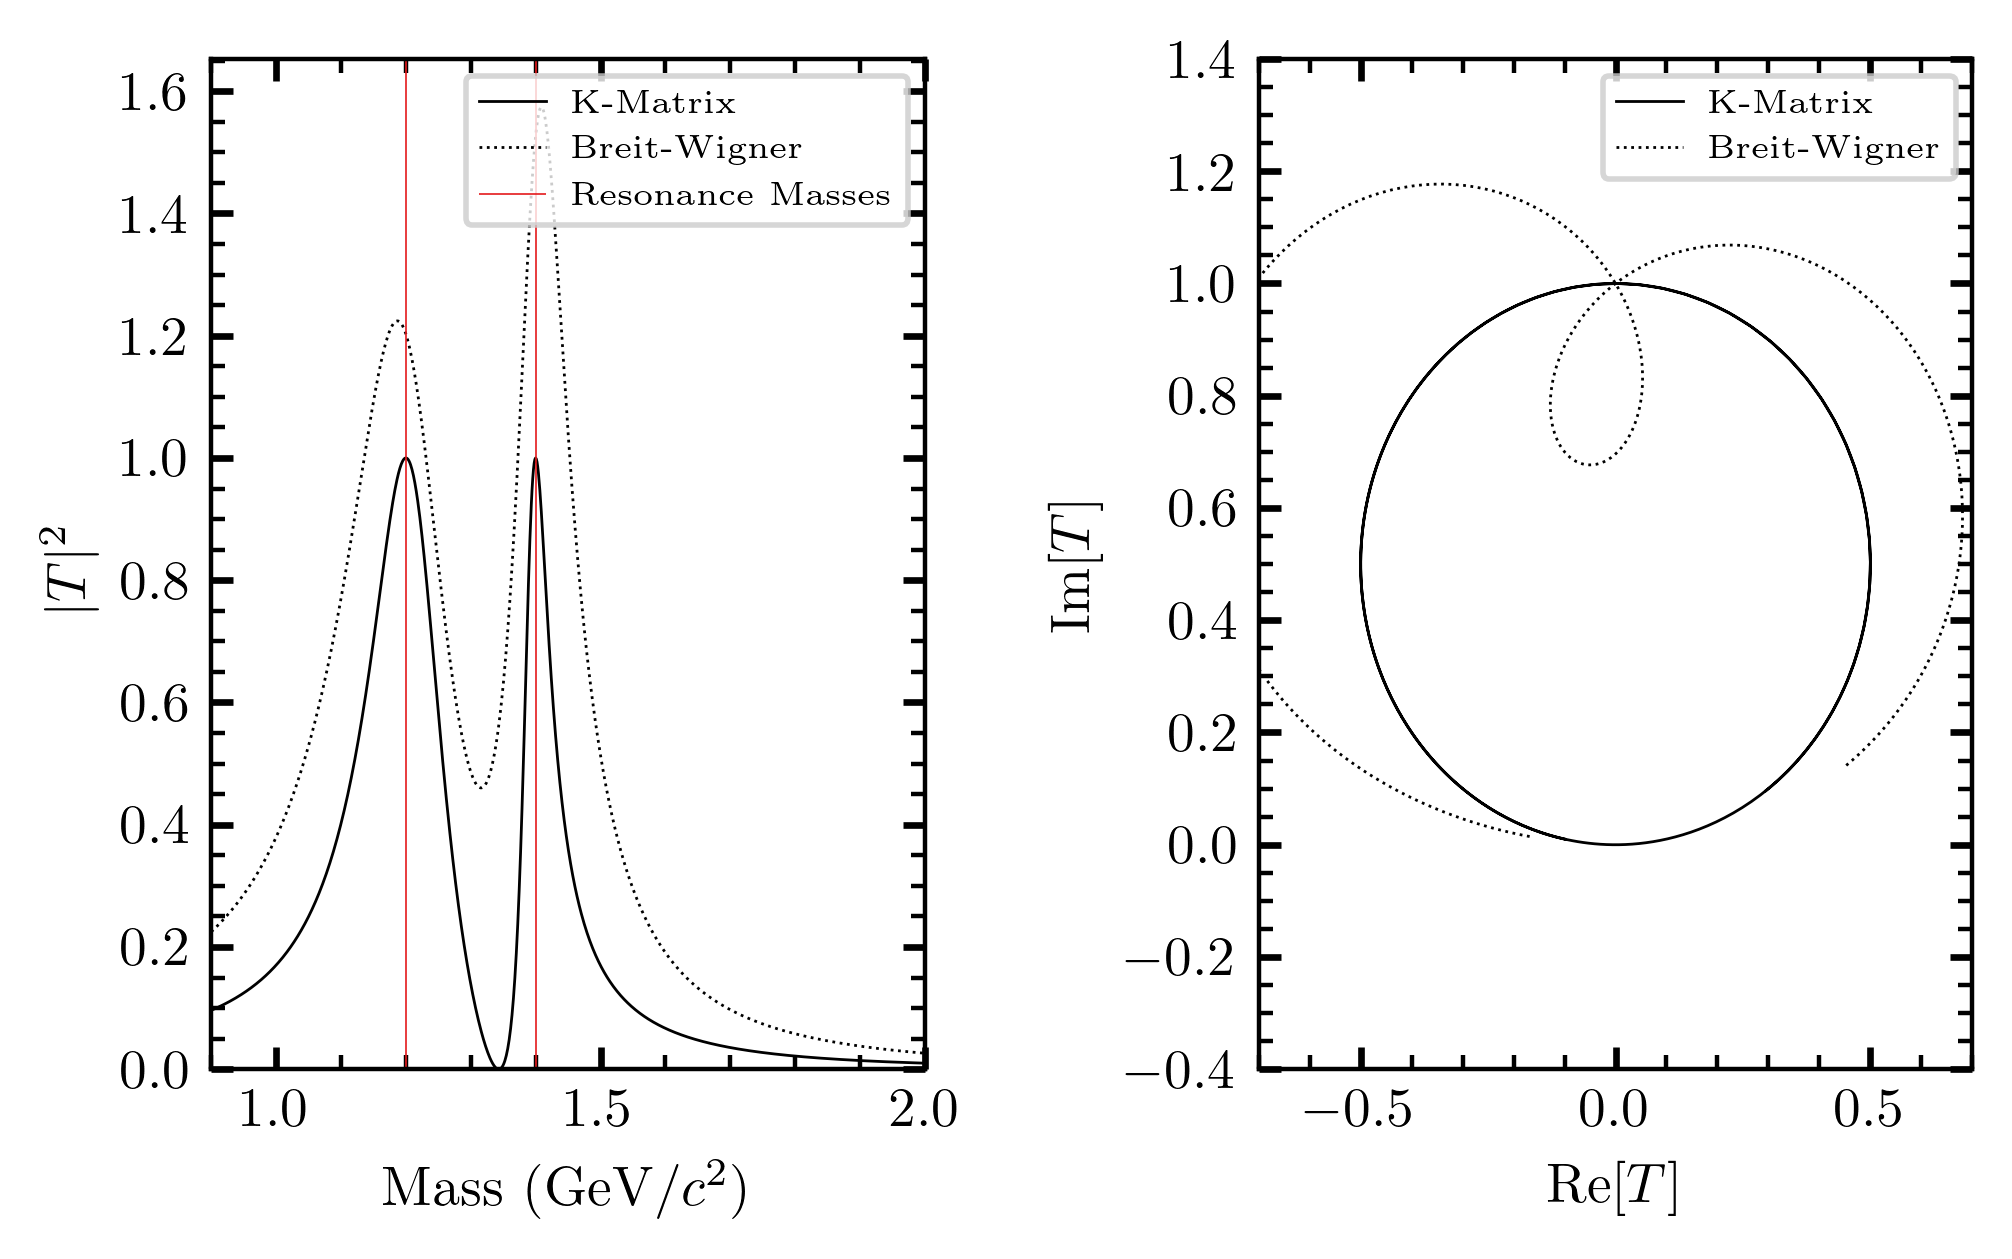
\includegraphics[width=0.8\textwidth]{figures/argand_diagram.png}
  \end{center}
  \caption{An Argand diagram depicting two fictitious resonances with masses of $\SI{1.2}{\giga\eV}/c^2$ and $\SI{1.4}{\giga\eV}/c^2$ and widths of $\SI{200}{\mega\eV}/c^2$ and $\SI{100}{\mega\eV}/c^2$ respectively using both the $K$-matrix formalism and interfering Breit-Wigners. The $T$-matrix formed from Breit-Wigners exceeds the unitary circle, implying that this construction breaks unitarity, while the $K$-matrix does not.}\label{fig:argand-diagram}
\end{figure}

\subsection{Resonances as Poles of the $K$-matrix}

Resonances can be parametrized either as constant elements in the $K$-matrix, which are usually interpreted as ``molecular'' resonances resulting from the exchange of force-carrying bosons, or from poles, which are thought of as the resonances describing decaying hadrons~\cite{au_meson_1987}. While we are more interested in the second case, we will include a linear combination of poles and constant terms in the parameterization, as follows:

\begin{equation}
  K_{ij}(m) = \sum_{\alpha} \frac{g_{\alpha i}(m) g_{\alpha j}(m)}{m_\alpha^2 - m^2} + c_{ij}
  \label{eq:k-matrix-parameterization}
\end{equation}

Here, $\alpha$ indexes the resonances, with $m_\alpha$ corresponding to the pole mass\footnote{This is not necessarily the same value as the centroid of a Breit-Wigner fit to the same data.} of the $\alpha$th resonance and $g_{\alpha i}$ corresponding to a term coupling the $\alpha$th resonance to the $i$th decay channel. $c_{ij}$ denotes any constant terms mentioned in the previously.

For a single resonance in a single channel, we can write the $T$-matrix as

\begin{align}
  T &= K(I-\imath K)^{-1} \\
    &= \frac{\frac{g^2(m)}{m_\alpha^2 - m^2}}{1 - \imath \left(\frac{g^2(m)}{m_\alpha^2 - m^2}\right)} \\
    &= \frac{g^2(m)}{m_\alpha^2 - m^2 - \imath g^2(m)}
\end{align}

which we see is identical to the Breit-Wigner form given in \Cref{eq:breit-wigner} with $g^2(m) = m_\alpha\Gamma_\alpha(m)$\footnote{Here, $\Gamma$ depends on $m$, which is true for a relativistic form of the Breit-Wigner amplitude.}.

Furthermore, we can now demonstrate the fundamental reason why we need to use the $K$-matrix in lieu of Breit-Wigners when describing multiple overlapping resonances. \Cref{fig:argand-diagram} shows that, even in a single channel, two interfering Breit-Wigners do not preserve unitarity, while the corresponding $K$-matrix does.

In the case where a resonance can decay into multiple channels, we say that $\Gamma_\alpha(m) = \sum_i \Gamma_{\alpha i}(m)$ is the total width and $\Gamma_{\alpha i}(m)$ are called the partial widths. In the relativistic form of the Breit-Wigner (and the Lorentz-invariant form of the resulting $S$-matrix), widths (and therefore partial widths) are given by

\begin{equation}
  \Gamma_{\alpha i} = \gamma^2_{\alpha i} \Gamma_{\alpha} B^\ell_{\alpha i}(m) \sqrt{\rho_i(m)}
  \label{eq:partial-width}
\end{equation}

where $\gamma^2_{\alpha i}$ is the fraction of the total width\footnote{However, $\gamma_{\alpha i}$ may itself be negative so long as it is purely real.}, $\Gamma_\alpha$, which is coupled to the channel $i$, and $\rho_i(m)$ is the phase space factor

\begin{equation}
  \rho_i(m) = \sqrt{\chi^+_i(m)\chi^-_i(m)}\quad\text{where}\quad\chi^{\pm}_i = 1 - \left(\frac{m_1 \pm m_2}{m}\right)^2
  \label{eq:rho}
\end{equation}

when the $i$th channel describes the decay $\alpha \to 1 + 2$ and $B^\ell_{\alpha i}(m)$ is the centrifugal barrier factor describing the suppression to the partial width when a resonance has angular momentum $\ell$. We typically parameterize this via form factors derived by Blatt and Weisskopf~\cite{blatt_theoretical_1979},

\begin{align}
  B^\ell_{\alpha i}(m) &= \frac{F_\ell(z_i(m))}{F_\ell(z_i(m_\alpha))} \\
  z_i(m) &\equiv \left(\frac{q_i(m)}{q_R}\right)^2 \\
  F_0(z) &= 1 \\
  F_1(z) &= \sqrt{\frac{2z}{z+1}} \\
  F_2(z) &= \sqrt{\frac{13z^2}{(z-3)^2 + 9z}} \\
  F_\ell(z) &= \sqrt{\frac{\abs{h_\ell^{(1)}(1)}^2}{z\abs{h_\ell^{(1)}(\sqrt{z})}^2}}
\end{align}

where $q_i(m) = m\rho_i(m)/2$ is the breakup momentum for the $i$th channel\footnote{i.e. the magnitude of the momentum either decay product will have in the rest frame of the decay}, $q_R$ is the impact parameter/interaction radius (we use $\SI{0.1973}{\giga\eV}$ in our calculations), and $h_\ell^{(1)}$ is a spherical Hankel function of the first kind (see Equation 2.4 of \cite{von_hippel_centrifugal-barrier_1972})

For clarity, we typically reparameterize these partial widths such that

\begin{equation}
  g_{\alpha i}(m) = g_{\alpha i}B^\ell_{\alpha i}(m)\sqrt{\rho_i(m)}
  \label{eq:coupling-expansion}
\end{equation}

so we can define the Lorentz-invariant $K$-matrix, $\hat{K}$, as

\begin{align}
  K_{ij}(m) &= \sqrt{\rho_i(m)}\left(\sum_{\alpha}B^\ell_{\alpha i}(m)\left[\frac{g_{\alpha i}g_{\alpha j}}{m_\alpha^2 - m^2} + \sum_n \bar{c}_{nij} m^{2n}\right]B^\ell_{\alpha j}\right)\sqrt{\rho_j(m)} \notag\\
  K_{ij}(m) &= \sqrt{\rho_i(m)} \hat{K}_{ij}(m) \sqrt{\rho_j(m)} \\
  \label{eq:invariant-k-matrix}
\end{align}

where we have absorbed some multiplicative factors into $c_{ij}$ to form the series expansion over powers of $m^2$ (since $\rho(m)$ and $B^\ell_{\alpha i}(m)$ only contain even powers of $m$) with coefficients $\bar{c}_{ij}$. Here, $\bar{K}$ replaces $K$ in \Cref{eq:t-matrix-from-k-matrix} as an intermediate step to defining a Lorentz-invariant formulation.

According to Chung\cite{chung_spin_1971}, the Lorentz-invariant form of the $T$-matrix, $\hat{T}$ can be written as

\begin{equation}
  T = \sqrt{\rho}\hat{T}\sqrt{\rho}
\end{equation}

where we define the notation

\begin{align}
  \rho_{ij}(m) &\equiv \rho_i(m)\delta_{ij}\\
  \sqrt{\rho_{ij}(m)} &\equiv \sqrt{\rho_i(m)}\delta_{ij}
\end{align}

In terms of \Cref{eq:t-matrix-from-k-matrix,eq:invariant-k-matrix,eq:k-t-inverse-relation}, we can write

\begin{equation}
  \hat{K}^{-1} = \hat{T}^{-1} + \imath \rho
\end{equation}

Following the previous derivation with these invariant forms, we find that

\begin{equation}
  \hat{T} = (I - \imath\hat{K}\rho)^{-1}\hat{K}
  \label{eq:t-matrix-from-k-matrix-invariant}
\end{equation}


\subsubsection{Production Amplitudes from a $K$-Matrix}

The $T$-matrix given in \Cref{eq:t-matrix-from-k-matrix-invariant} describes $s$-channel resonances (as in $a + b \to X \to c + d$). We can transform this into a production amplitude following Aitchison~\cite{aitchison_k-matrix_1972}:

\begin{equation}
  \hat{F} = (I - \imath\hat{K}\rho)^{-1}\hat{P}
  \label{eq:k-matrix-production-amplitude}
\end{equation}
where
\begin{equation}
  \hat{P}_i(\vec{\beta}; m) = \sum_\alpha \left(\frac{\beta_\alpha g_{\alpha i}}{m_\alpha^2 - m^2} + \sum_n c_{ni} m^{2n} \right)B_{\alpha i}^{\ell}(m)
  \label{eq:p-vector}
\end{equation}

Here, $\beta_\alpha$ describes the complex coupling from the initial state to the resonance $\alpha$. This can be thought of like a coupling coefficient in front of a single Breit-Wigner. The polynomial of coefficients are included for completeness, as any constant terms in $P$ preserve unitarity in the same way as constant terms in $K$, and the division of the factor of $\rho_i(m) \sim \rho_i(m^2)$ from \Cref{eq:coupling-expansion} and $B^\ell_{\alpha i}(m) \sim B^\ell_{\alpha i}(m^2)$ creates the given form.

\subsubsection{The Chew-Mandelstam Matrix}

For reasons which will become clear, we will define the diagonal matrix $C$, called the Chew-Mandelstam matrix, with the property

\begin{equation}
  \Im[C(m)] = -\rho(m)\quad\text{or}\quad C(m) = A(m) - \imath\rho(m)
\end{equation}
for some real function $A(m)$. It can be shown that we can replace $-\imath\rho$ in \Cref{eq:t-matrix-from-k-matrix-invariant} with such a matrix $C$ and still retain a valid $K$-matrix representation~\cite{wilson_resonances_2015},

\begin{equation}
  \hat{T} = (I + \hat{K}C)^{-1}\hat{K}
\end{equation}

and

\begin{equation}
  \hat{F} = (I + \hat{K}C)^{-1}\hat{P}
  \label{eq:k-matrix-production-amplitude-chew}
\end{equation}

The exact form of $A(m)$ is arbitrary, but we will be using

\begin{equation}
  C_{ii}(m) = C((m_1 + m_2)^2) + \frac{\rho_i(m)}{\pi}\ln\left[\frac{\chi^+_i(m) + \rho_i(m)}{\chi^+_i(m) - \rho_i(m)}\right] - \frac{\chi^+_i(m)}{\pi}\frac{m_2 - m_1}{m_1 + m_2}\ln\frac{m_2}{m_1}
  \label{eq:chew-mandelstam}
\end{equation}

where $m_1$ and $m_2$ are the masses of the final state of the $i$th decay channel, and we can choose $C((m_1 + m_2)^2) = 0$ for normalization. See \cite{oller_nd_1999}, \cite{basdevant_unitary_1977}, \cite{oller_chiral_2001}, and \cite{reid_generating_1984} for derivations and additional details of this expression. The motivation for this choice is that it behaves better below threshold than $\rho(m)$, as can be seen in \Cref{fig:chew-mandelstam}.

\begin{figure}
  \begin{center}
    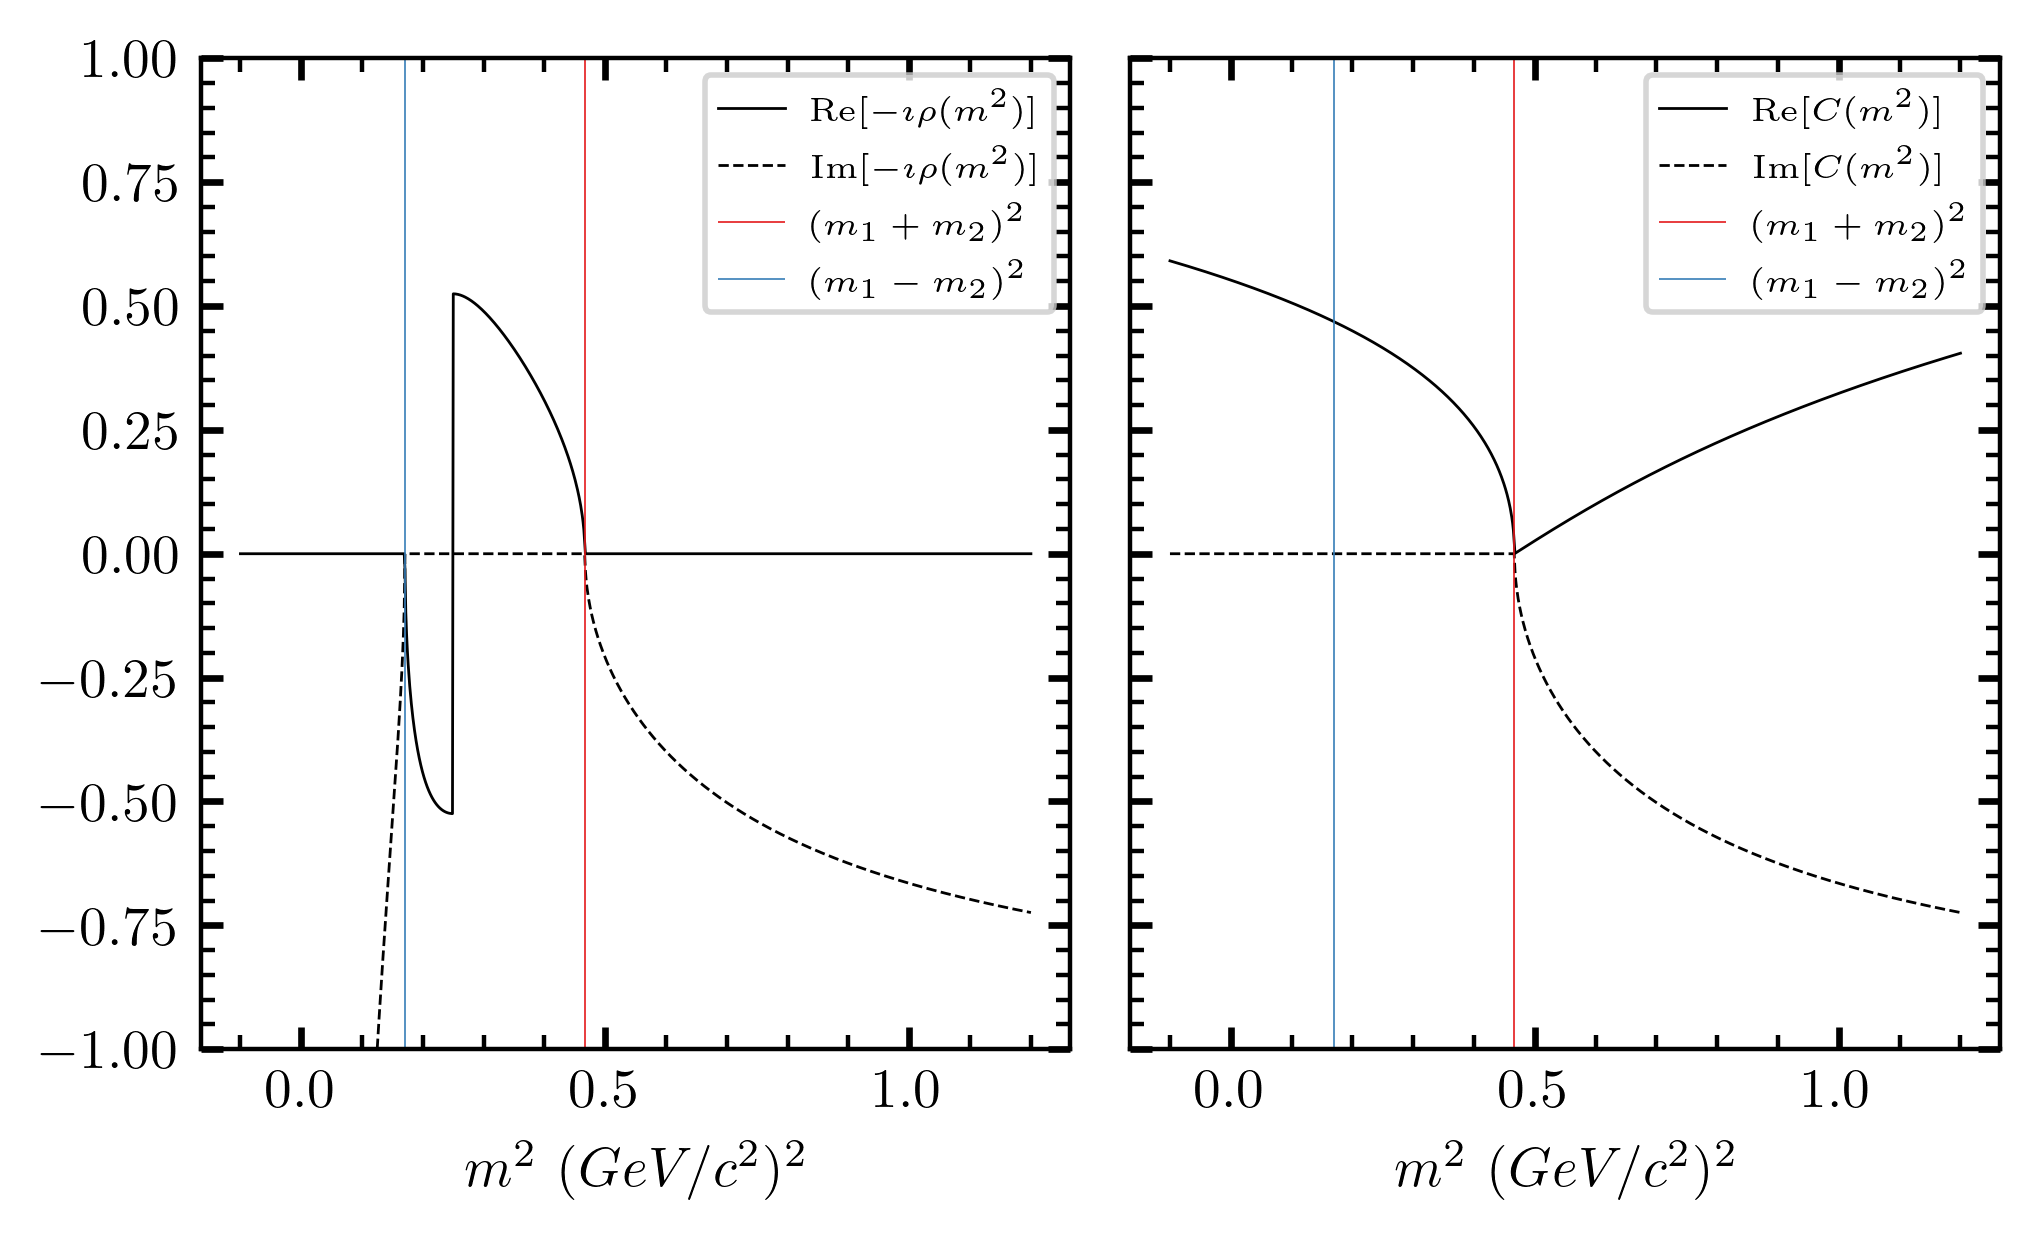
\includegraphics[width=0.8\textwidth]{figures/chew_mandelstam.png}
  \end{center}
  \caption{A comparison of the normal phase-space function, $\rho(m)$ (left) and the Chew-Mandelstam matrix, $C(m)$ (right) on the $\pi^0\eta$ channel. Both functions have the same imaginary part above the threshold $m = m_1 + m_2$, but phase-space function has a branch cut at $m^2 = \frac{(m_1^2 - m_2^2)^2}{m_1^2 + m_2^2}$ (the jump in the left plot between the red and blue lines) as well as a discontinuity at $m^2 = (m_1 - m_2)^2$ in both real and imaginary parts.}\label{fig:chew-mandelstam}
\end{figure}


The impetus of this complication is that this particular formulation of the Chew-Mandelstam matrix is used in \cite{albrecht_coupled_2020} and \cite{kopf_investigation_2021}. We do not have enough data to constrain the pole positions of every resonance in this channel (as we only have access to one of several channels used in those papers), so we will use the $K$-matrix coefficients ($g_{i\alpha}$ and $m_\alpha$) from their coupled-channel analysis of data from the Crystal Barrel and COMPASS experiments as fixed values in our analysis, fitting only the couplings ($\vec{\beta}$) to photoproduction. Additionally, using the results from these papers requires a Adler zero term in front of the $K$-matrix for the $f_0$ mesons of the form $\frac{(s - s_0)}{s_\text{norm}}$, where they use $s_0 = m^2_{\pi_0}/2$ and $s_\text{norm} = 1$.

We can then combine \Cref{eq:k-matrix-production-amplitude-chew} with \Cref{eq:generalized-polarized-intensity}, choosing $T^{J(\epsilon)}_{M;\eta}(\vec{\beta}; m) = \hat{F}(\vec{\beta}; m)$, to form a mass-dependent model of polarized photoproduction for the $K_S^0K_S^0$ channel which will be further discussed in \Cref{sec:mass-dependent-fits}.

\section{Waveset Selection}

\chapter{Results and Systematic Studies}
\section{Mass-Independent Fits}
\section{Mass-Dependent Fits}
\section{Systematics}
\chapter{Conclusion}

\appendix
\chapter{Derivation of the Chew-Mandelstam Function}
We begin with the dispersion integral\footnote{see \href{https://arxiv.org/pdf/1411.2004.pdf}{arXiv paper}}:
\begin{equation}
  C(s) = C(s_\text{thr}) - \frac{s - s_\text{thr}}{\pi} \int_{s_\text{thr}}^{\infty} \dd{s'} \frac{\rho(s')}{(s' - s)(s' - s_\text{thr})}
\end{equation}
where $s_\text{thr} = (m_1 + m_2)^2$ and
\begin{equation}
  \rho(s) = \sqrt{\left(1 - \frac{(m_1 + m_2)^2}{s}\right)\left(1 - \frac{(m_1 - m_2)^2}{s}\right)}
\end{equation}

We first focus on just the integral part:
\begin{equation}
  I(s) = \int_{s_\text{thr}}^{\infty} \dd{s'} \frac{\rho(s')}{(s' - s)(s'-s_\text{thr})}
\end{equation}

\begin{equation}
  \lim_{\epsilon\to 0}\int_a^b \dd{x} \frac{f(x)}{(x-x_0) + \imath\epsilon} = \fint_a^b \dd{x} \frac{f(x)}{(x-x_0)} + \imath\pi f(x_0)
\end{equation}

\begin{align}
  I(s) &= \fint_{s_\text{thr}}^{\infty} 
\end{align}


\backmatter
\printbibliography
\newpage
\end{document}
